\documentclass{kuee}
\renewcommand{\include}[1]{}
\renewcommand\documentclass[2][]{}
\usepackage[dvipdfmx]{graphicx}
\usepackage{amsmath}
\usepackage{url}

\title{表現型特徴ネットワーク解析におけるGroup-In-a-Boxレイアウトの有効性評価}
\etitle{Evaluation of Group-In-a-Box layouts in the analysis of phenotype network}
\author{青山 望}
\eauthor{Nozomi Aoyama}
\professor{小山田 耕二 教授}
\course{京都大学大学院工学研究科}
\department{電気工学専攻}
\date{令和2年1月31日}

%%% 本文
\begin{document}
\maketitle      % 表題を出力
\begin{eabstract}   % 英文要旨を出力
Network analysis is a recent common method in biology so that researchers figure out the mechanism of animal development.
Biology network often has group structure within the graph that is called complexity; hence, the network data require a special technique to be visualized.
GIB (Group-In-a-Box) layout is a graph-drawing method for complex network and is knows as effective.
However, its four variants, ST-GIB, CD-GIB, FD-GIB, and TR-GIB, have not been evaluated thoroughly.
In this study, we aim to reveal which layout of GIB is the best layout for visualizing complex network with two user studies.
We utilize four tasks in the first experiment to evaluate GIB variants from various perspectives.
In the second task, path finding is adopted to discuss the capabilities of GIBs in more detail with considering their data scalabilities.
We also focus on which visual attribute in a graph affects the readability by using an eye tracking system, which allows us to have insights about why task results differ.
TR-GIB has turned out to be the most effective layout in the network analysis, while there is a trade-off relation between itself and FD-GIB.
Domain experts provide us interesting comments on the effectivity of each GIB, which support our result.
We also reveal several visual attributes that have influences on the readability such as the orderly arrangement of groups, and the angles of edges, and so on.
Our findings might enhance the quality of complex network analysis, and our results provide new insights into designing graph drawing methods.
\end{eabstract}
\tableofcontents    % 目次を出力
{}
\chapter{序章}
\label{chap:intro}

生命は生化学現象を基盤とし,遺伝子やmRNA,タンパク質,表現型特徴などの異なるスケールで制御される複雑系からなる.
この生命現象を理解するためには,現象のダイナミクスや異なるスケール間の相互作用を具に観察する必要がある.
ここ十数年で, 顕微鏡により細胞の時空間動態を自動的に計測するバイオイメージ・インフォマティクス技術が発達し,大量の生命科学データが取得されている.
増え続ける生物学データを有効に利用し新たな生物学的知見を得るため, データ駆動型科学がその重要性を増している,
% それを支援するためには,異種のデータを如何に見るかという点を考える必要がある.
ここでデータ駆動型科学とは,事前の仮説無しにデータから何が言えるのかを考え,科学的手法における仮説生成をデータに基づき行うアプローチのことを指す.
生物学データとその解析に可視化技術を統合させるアプローチが,データ駆動型科学の基礎となるユーザー主導型のデータ探索を促進させうる.

生物学データのうち特に情報可視化技術を必要とするものは,タンパク質間相互作用や遺伝子の共発現情報,表現型特徴関係のような関係性データである.
ここで表現型特徴とは生物の示す外見上の形態的, 生理的特徴のことである.
特に遺伝子ネットワークや表現型特徴ネットワークのように,複雑なネットワーク構造を有するデータを効果的に可視化することはデータ理解や新たな仮説構築を促す.
我々の共同研究者である理化学研究所の研究グループは,現在線虫C. elegansの初期発生を研究しており,初期の細胞分裂においての細胞核の大きさや分裂軸の角度など,線虫の表現型特徴を定量化している.
それら表現型特徴間の関係性を表現型特徴ネットワークとして表し, ネットワーク解析により生物学的な因果関係を示唆する関係性を抽出することを目指している.
これらの研究を通じて,線虫の発生メカニズムが解き明かされれば,人間を含めたその他の生物の発生メカニズムを紐解く手がかりとなり,ひいてはがん研究や再生医療といった分野への貢献が期待できる.

図\ref{fig:example_phenotype}, \ref{fig:64-origin-layout}に表現系特徴間の相関関係を可視化したネットワークを示す.
ノードは表現型特徴を表し,エッジは表現型特徴の相関関係を表す.
表現型特徴は細胞ごとに定義されるため,同一細胞の表現型特徴ノードをグループ化していて,グループをその分裂期ごとに配置することでどの分裂期の特徴であるか見分けやすいようなレイアウトとなっている.
生物学者はこのようなネットワークから特徴的な関係性を抽出しようと試みているが,図\ref{fig:example_phenotype}, \ref{fig:64-origin-layout}ではエッジの重なりや交差が多く,この状態ではネットワーク解析が極めて困難になる.
このような問題に対してはグラフ描画レイアウトや粗視化技術に代表される情報可視化の技術が有効である.
例えば隣接行列は関係性データを可視化する手法の一つであり,関係性の多さから起こるエッジ交差などの視覚的問題が生じずにノードを適切に並べ替えることでグループ構造の検出が容易であるというメリットを持つが,複数ノード間の繋がりが理解しにくい,
ノードの配置に位置情報を反映できないなどのデメリットがある.
一方でノードリンクグラフはノード間の関係性を直観的に理解しやすく,ある程度のサイズまではハブやクラスタなどの重要なネットワーク指標も視認しやすいが, 密なグラフにはレイアウトの工夫無しにはエッジ交差が多く扱いづらいものになる.
このように各可視化手法には向き不向きがあることから,表現型特徴ネットワークにもそれに適した可視化手法を用いることが求められている.

先述した通り,表現型特徴ネットワークはグループ構造を有するネットワークである.
グループ構造を有するネットワークの可視化手法はVehlowらの調査論文に体系化されている\cite{Vehlow2017VisualizingGS}.
グループ構造の表現方法には,ノードの色で属するグループを表現するもの,グループ構造をネットワークと別に明示するもの,ノードリンクグラフの中でグループ内のつながりを遷移行列で表すもの,グループ毎にノードを円や四角形で囲うものなどがある.
このうち, ノードの色でグループ構造を表すものはグループやノードの数が増えた際に配色や識別が難しくなるという欠点がある.
遷移行列を埋め込んだ表現はグループ間の繋がりや複数ノード間の接続が理解しにくく表現型特徴ネットワークに適さない.
グループ毎に属するノードを図形で囲うという方法は,グループ構造のみならずエッジの情報など様々な要因を考慮してレイアウトができるため有効だと考えられ,その中でも同一グループに属するノードを四角形で囲むレイアウトを共同研究者らは使用してきた.
この可視化手法はGroup-In-a-Box(GIB)レイアウトと呼ばれる.GIB は各グループに属するノードがノード数に比例した大きさの箱に囲まれており,グループ内のネットワーク,グループ間のネットワーク,グループの大きさを同時に表現できるという特徴がある.
GIBは表現型特徴ネットワークを表すのに望ましいレイアウトであり, 効果的なネットワーク解析を促せると考えられる.

GIBレイアウトはグループを囲む箱をどのように配置するかという観点で,図\ref{fig:example_GIB}に示されるようにいくつかの手法が提案されている.
GIBレイアウトについて,計算的実験\cite{chaturvedi2014group,onoue2017optimal}によりGIB が評価されているが,我々の知る限りユーザー実験によりGIB を評価した研究は未だ存在しない.
いくつかの計算可能な指標がグラフの可読性に影響することが分かっている\cite{468391,purchase1997aesthetic,purchase1998performance,purchase2002empirical,giacomo}が,グラフの理解には人間の認知の観点からも様々な未解明の要因が影響するため,真にユーザーが利用しやすいGIBレイアウトがどれかは分かっていない.
そこで本研究では,二種類のユーザー実験を行い,どのGIBレイアウトがネットワーク解析に最も有効か,また表現型特徴ネットワークに代表される実応用の場面でどのレイアウトを用いるべきかを明らかにする.

一つ目の実験では,先行研究\cite{Vehlow2017VisualizingGS,saket2014group}で報告されているタスク分類をもとに比較的簡単な4種類のタスクを設定し, 4種類のGIBレイアウトの有効性を概略的に評価することを目的とする.
実験では,正答率と完了時間を計測することでレイアウト間のタスク性能の優劣を比較した.
これに加え,視線追跡システムを利用し実験中の被験者の視線データを記録した.
視線追跡システムは,視覚認知やヒューマンコンピューターインタラクションの分野でよく用いられる.
実験中の視線データを解析することで,タスク性能の優劣がなぜ生まれたかについて議論することができる\cite{andrienko2012visual,duchowski2007eye,kurzhals2014evaluating}.
具体的には,ネットワークグラフにおけるどの視覚特徴が被験者のパフォーマンスに影響したかを特定することを目指す.
二つ目の実験では,一つ目の実験で好成績を残した二つのレイアウトに着目し,より実際の解析作業に近いデータとパス探索のタスクを用いることで, どちらのレイアウトが最良であるかを明らかにし, 加えてそれらのデータ拡張性も議論する.

本研究では上述した二種類のユーザー実験と共同研究者である2名の生物学者からのフィードバックをもとに,どのGIBレイアウトが表現型特徴ネットワークの解析に最も有効かを明らかにする.
また,視線追跡データを解析することにより,ネットワーク可視化において可読性に影響し得る視覚的特徴を特定する.
こうした特徴を発見できれば,GIBや他のグラフ描画手法の可読性を向上させるアイデアを得られ,グラフ可視化手法の改善に貢献することができる.

本稿の以降の構成は次のとおりである.まず第2章では本研究の背景と関連研究について説明する.
続いて第3章で実験1, 第4章で実験2について述べる.
第5章では実験結果についての専門家からのフィードバックを述べ, 最後に第6章で結論を述べる.

% 表現型特徴ネットワークにもそれに適した可視化手法を用いることが効率的な解析には必要である.
% また, 本研究は表現型特徴ネットワークの解析効率化に動機づけられたものであるが, GIBは他の複雑ネットワークにも利用可能な手法である.
% 上述したTwitterのようなSNSネットワークの他, 企業間取引ネットワークや交通ネットワークにも応用が可能である.
% 理化学研究所の研究員達は, 表現型特徴ネットワークと並行して遺伝子ネットワークの解析も進めており, これも遺伝子の分類によりグループ構造を持ちGIBの対象となる.
% 本研究で明らかになった最良のGIBはこうしたデータでも有効であると考えられる.


\begin{figure}
  \centering
  \includegraphics[width=15cm]{./images/PhenotypeNet.png}
  \caption{表現型特徴ネットワークの例. 8細胞期までの細胞に観察された421の表現型特徴とそれらの相関関係をネットワークとして表したもの. グループは表現型が属する細胞と細胞の現れる細胞期により決定される. \label{fig:example_phenotype}}
\end{figure}

\begin{figure}
  \centering
  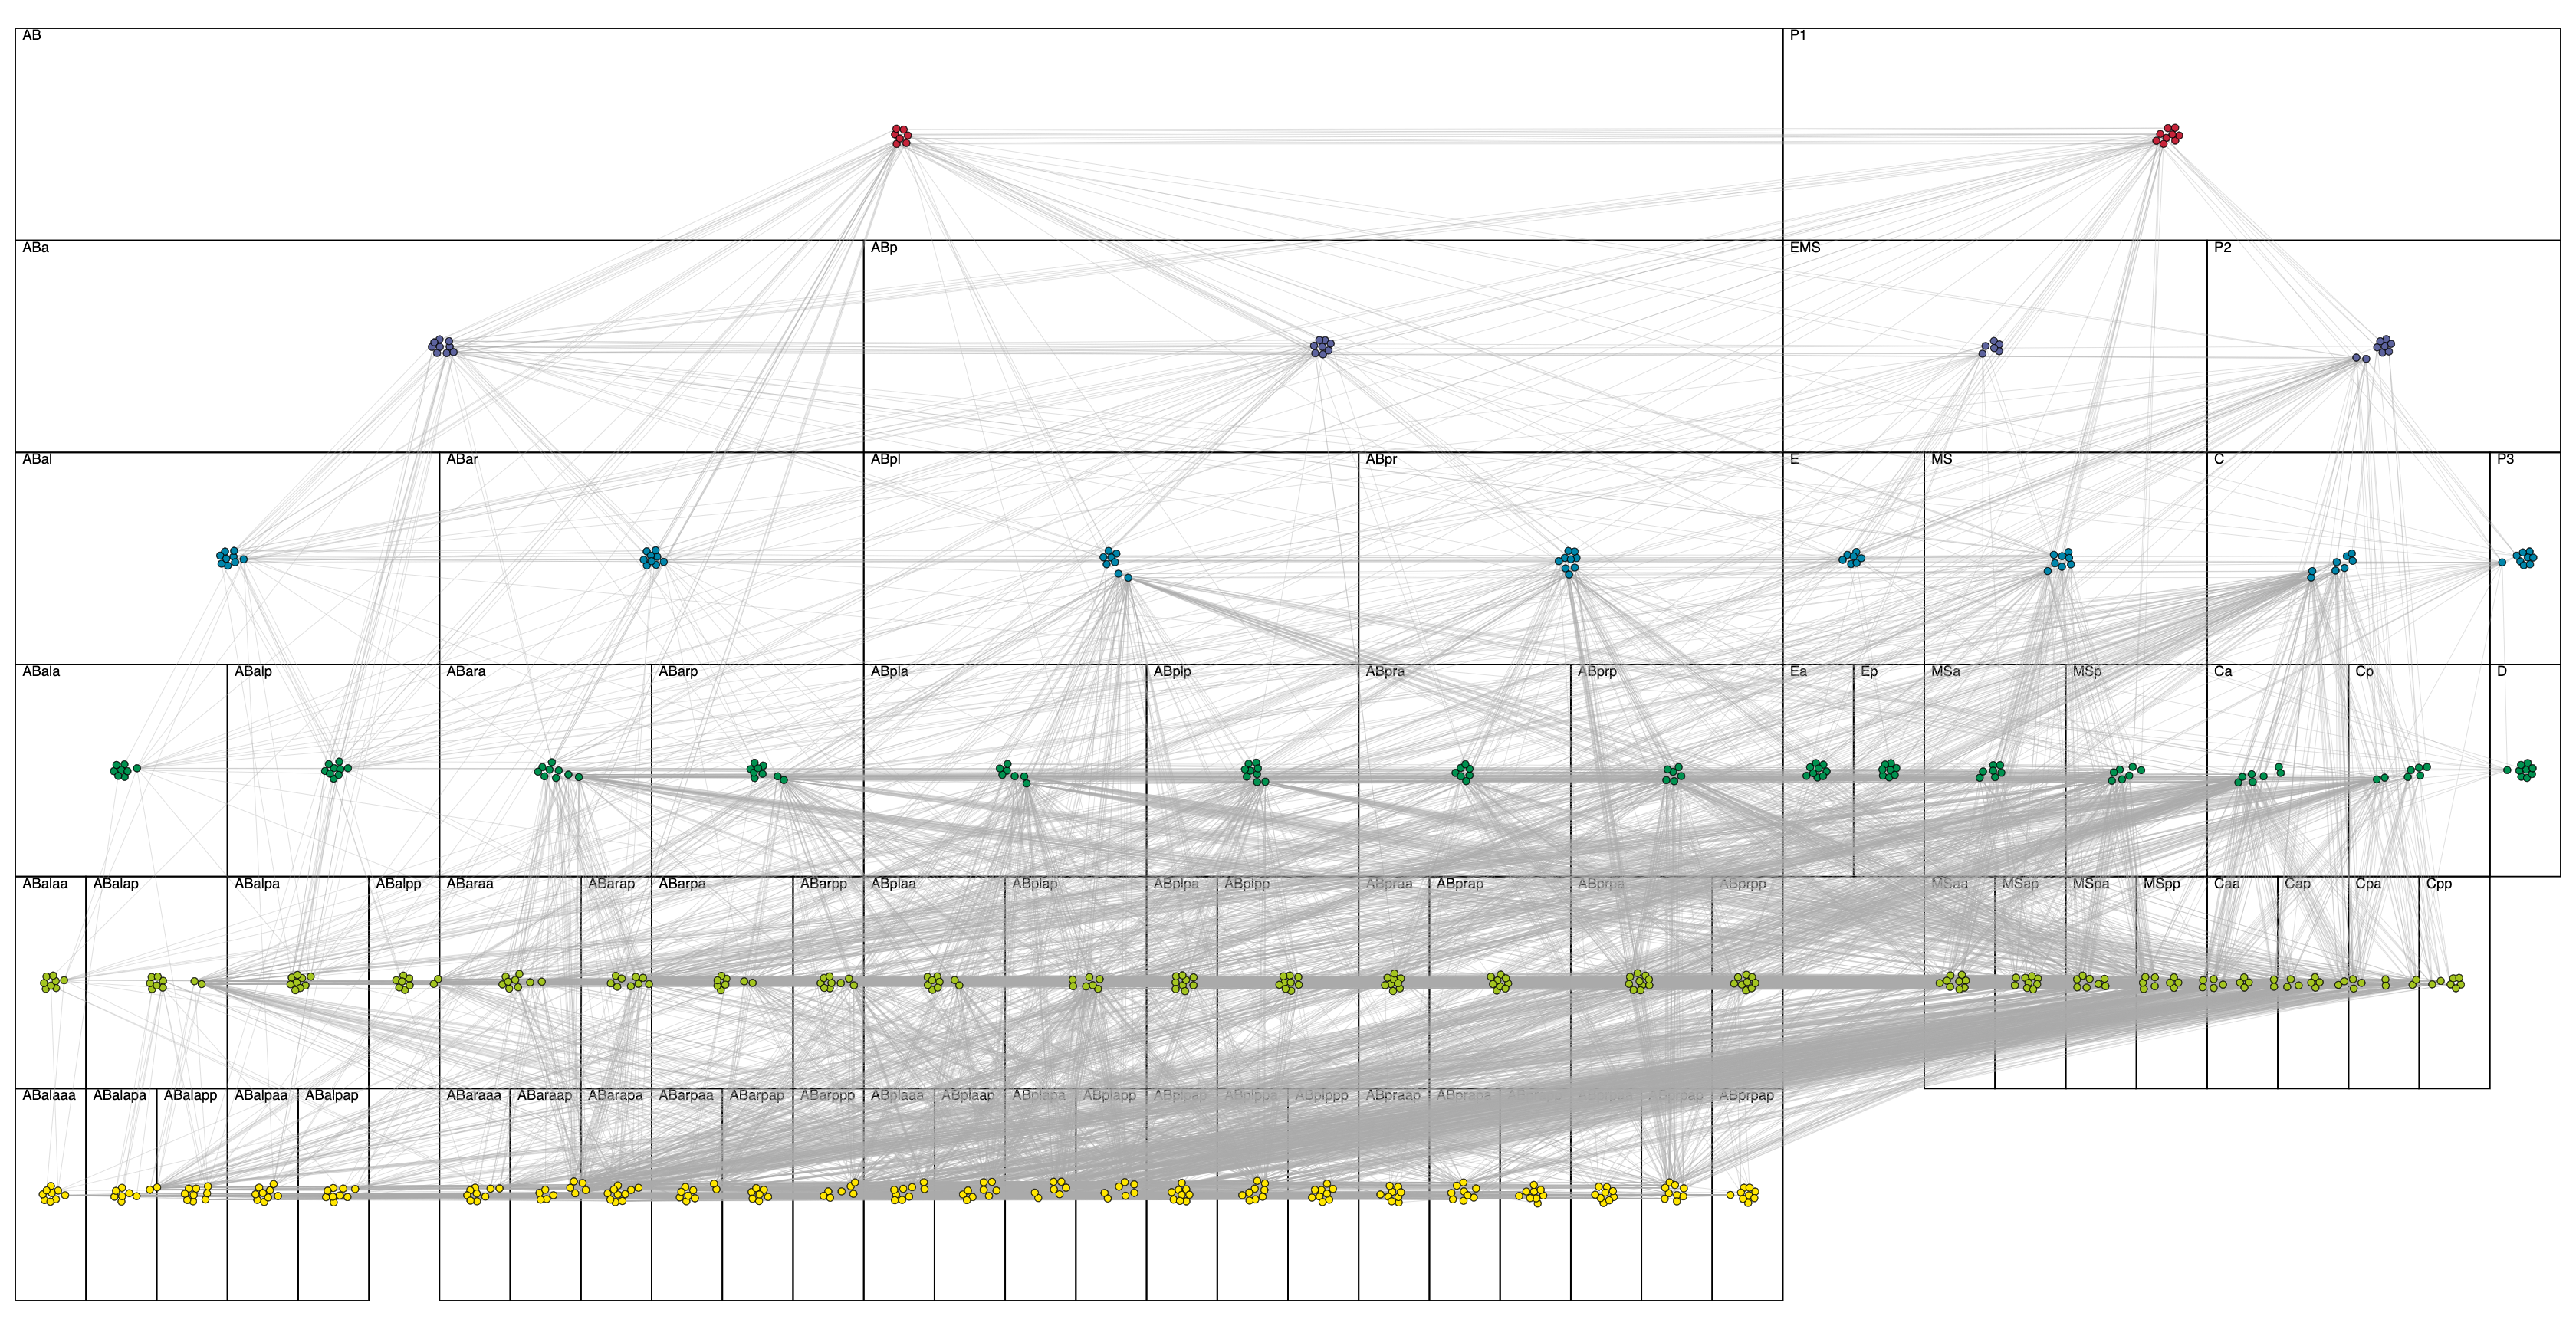
\includegraphics[width=15cm]{./images/azuma_threshold08.png}
  \caption{64細胞期までの表現型特徴ネットワーク. グループは細胞期毎に上から下に配置されている.発生が進むにつれグループの数が増え, エッジの密度が上がり視認が難しくなる. \label{fig:64-origin-layout}}
\end{figure}

\begin{figure}
  \centering
  \includegraphics[width=15cm]{./images/examples.png}
  \caption{GIBレイアウトの種類. (a)ST-GIB, (b)CD-GIB, (c)FD-GIB, (d)TR-GIB. 4種類のグラフは同じデータを可視化したものである. \label{fig:example_GIB}}
\end{figure}


\chapter{関連研究}
\label{chap:relatedwork}
本章では関連研究について記述する.
\ref{sec:vis_bio}節では研究の動機となった表現型特徴ネットワークについて説明する.
\ref{sec:graph_for_group_structure}節ではグループ構造を持つネットワークの可視化手法について述べる.
% 該当する手法はいくつかあるが, その中でのGIBの立ち位置と, なぜGIBを研究対象にしたかを詳細に説明する.
\ref{sec:GIB}節では本研究で対象とする4種類のGIBについて述べる.
\ref{sec:evaluation_with_eyetracking}節では視線追跡グシステムを用いた可視化の評価研究について記述する.
% 可視化の評価研究は近年その重要性を高めており, その中でも視線追跡システムを用いた評価は可視化利用時のユーザーの行動をより定量的に述べられる上更なる考察を与えられるために注目されている.
% 一方で, 高性能な視線追跡システムが一般に使用されるようになってから日が浅く, そのデータの膨大さから解析方法もあまり整っていない.
% 関連研究を述べることで, 本研究の目的に即した視線データ解析を目指す.

\section{表現型特徴ネットワーク}
\label{sec:vis_bio}
動画像に画像認識技術を適用して生物特徴の動態を計測する技術であるバイオイメージインフォマティクスにより高スループットに生命動態を定量化できるようになり,大規模なデータベースが構築されている.
本研究ではモデル系として研究の進んだ多細胞生物である線虫C. elegansの初期発生における表現型特徴ネットワークを対象とする.
8細胞期までの表現型特徴ネットワークの構築については次の通りである.
まずC. elegansの発生中の正常な胚の細胞動態を微分干渉顕微鏡により4次元的に撮像した動画像を取得した.
撮像は0.5$\mu$mごとに66スライス計測され,20秒ごとに360回,計2時間計測された.取得した動画像データに対して画像認識プログラムを適用し,核の大きさ,核の位置,核間の距離,核の形状,紡錘体の位置,向き等の胚の表現型特徴の動態を計測する.
野生胚33個体において1 - 8細胞期までの各細胞に対して上述の表現型特徴を定量化することで,計421の表現型特徴を抽出した.
次に計測された表現型特徴間のピアソンの相関係数を計算することで,表現型特徴間の関係性から図\ref{fig:example_phenotype}のように表現型特徴ネットワークが構築される.
ここでノードは表現型特徴を表し,リンクは表現型特徴相関を表す.
このように表現型特徴を構築することで線虫の初期発生においてどの特徴とどの特徴に関連があるのかを推察することができる.
同様な手法で, 64細胞期までの各細胞に対してもデータを記録し, 図\ref{fig:64-origin-layout}に示されるネットワークが得られている.
これらのネットワークの構築は理化学研究所の共同研究者により行われた.

\section{グループ構造を有するネットワークの可視化}
\label{sec:graph_for_group_structure}
データの重要性が広く認知されている近年では, 頻繁なデータ収集や計測技術の発展によりネットワークデータはその量も複雑性も増している.
ネットワークの膨大さと複雑さに対応するため, グラフ描画の分野では様々な手法が提案されてきた.
Eadesらはforce-directed layoutと呼ばれる手法を提案した\cite{eades84}.
この手法では, ノード間の斥力, エッジ間の引力, そしてスクリーン中央からの引力によって各ノードが配置される.
エッジが引力を持つことから, 関係するノード同士が近くに配置され, エッジの長さが短くなる.
見た目が美しくグラフのトポロジーが理解しやすいことから, このレイアウトは広く利用されいて\cite{Kobourov2013ForceDirectedDA}, いくつかの計算アルゴリズムが存在する\cite{harel2000fast,koren2003drawing,hachul2004drawing}.
図\ref{fig:gene}に線虫における遺伝子細胞データのネットワークをforce-directedレイアウトで可視化したものを示す.

一方で, グループ構造を有するネットワークの可視化には専用に設計された可視化手法を用いるという動向がある.
大規模なネットワークデータでは, コミュニテイ検出の重要性は周知であり\cite{girvan2002community,newman2004detecting}, 先述した表現型ネットワークや遺伝子ネットワーク, さらにはソーシャルネットワークや交通ネットワークにもグループ構造が定義される.
こうしたネットワークの可視化にはいくつかの手法があるが, その多くはforce-directedレイアウトに基づいたものである.
最も典型的なグループ構造を表現する方法は, ノードを属するグループによって決まる色で描くものである\cite{mcpherson2005discovering}.
また, ノードの形をグループによって変化させるという方法も考えられる.
しかし, こうした方法は実際の大規模データ解析では効果的でないと知られている.

Vehlowらはグループ構造を有するネットワークの可視化手法に関する調査論文を発表している\cite{Vehlow2017VisualizingGS}.
彼女らは可視化手法の特徴やユーザー実験で用いられたタスクについて詳細に記述し, それぞれをいくつかのカテゴリに分類している.
可視化手法の分類は可視化手法とデータ構造の特徴により決まる.
前者はグループ構造が視覚的にどう表現されているかを表しており, その表現の仕方によってノード属性, 並置, 上書き, 埋め込みという4つの分類に分けられる.
後者はグループの重複性とグループ間の階層構造性が基準となる.
グループの重複性とはノードが同時に複数のグループに属することを指し, 階層構造性はある二つのグループに包含関係があることを示す.
Vehlowらは今までに提案されたグループ構造を有するネットワークの可視化手法をそれぞれのカテゴリに分けて紹介している.

GIBレイアウトもグループ構造を有するネットワークを可視化する手法の一つである\cite{chaturvedi2014group,onoue2017optimal,rodrigues2011group}.
GIBには主に4つの種類(ST-GIB, CD-GIB, FD-GIB, TR-GIB)があり, 本研究ではこれらを対象として比較実験を行う.
GIBはそれぞれのグループにスクリーン画面を割り当てて個別に描画できるため, 同一グループ内のネットワークを観察することが容易になる.
またグループを囲う箱の面積がグループに属するノードの数に比例しているため, グループの大きさも表現することができる.
Vehlowらの分類においては, GIBは上書き, 重複性無し, 階層構造性無しというカテゴリに分類され, 表現型ネットワークの
可視化に適したものである.
このカテゴリに属する可視化手法はいくつか紹介されていて\cite{chaturvedi2014group,henry2007nodetrix,shneiderman2006network,bach2013graphdiaries,dekker2001visualisation}, グループ情報の符号化に色のみを用いるものや, グループ情報をネットワークと分離して表現するもの, さらにグループ内構造の表現に遷移行列をグループ構造を表現する埋め込んだ可視化方法が存在する.
しかし表現型特徴ネットワークを表す上では,細胞の数だけ増え得るグループの数に対応が難しく,特徴間のつながりやグループ関係が直観的に把握できないこれらの方法は望ましくない.
一方で, 同一グループを図形で囲う上書き方式は表現型特徴ネットワークに対応可能であり, その中でも計算的にグループの配置を調整しやすい四角形で囲んだもの, 即ちGIBが最も有効であると考えられる.

\begin{figure}
  \centering
  \includegraphics[width=15cm]{./images/nucmen.png}
  \caption{Force-directedレイアウトで描画された核膜に関わる遺伝子ネットワーク.遺伝子ネットワークを形成する遺伝子間相互作用は, タンパク質間や遺伝子共発現情報などを基に定量化している. \label{fig:gene}}
\end{figure}

\section{GIBレイアウト}
\label{sec:GIB}
GIBには少なくとも4種類が存在し, そのうちいくつかは計算的指標により評価がされている.
ChaturvediらはST-GIB, CD-GIB, FD-GIBの三種を309のTwitterネットワークを用いて, エッジと箱の交差数, スクリーン画面の使用効率, 計算時間, 平均の箱のアスペクト比を計算することにより比較した\cite{chaturvedi2014group}.
また予備実験としてST-GIBとCD-GIBを対象に小規模な予備実験を行なった.
% またその予備実験として, ST-GIBとCD-GIBを対象に9人の被験者を用いてレイアウトの使いやすさを0 - 9のスコアで評価した.
% 予備実験ではCD-GIBの方が使いやすいと評価され,
計算実験では三種類のレイアウト間で以下のような結果が得られた.
FD-GIBはエッジと箱の交差数が少ないという利点があったが, スクリーン画面を浪費していた.
CD-GIBは計算時間が短く, ST-GIBはスクリーン画面の使用効率がよかった.
Chaturevediらの研究は有意義なものであるが, 予備実験はタスクにおいて精度などの指標を用いてない他, 計算実験では多数のエッジを一本にまとめて描いたグラフを使用していて信頼性に欠ける.
尾上と小山田は計算によりTR-GIBによりグループの近接性(重み付けたエッジの長さの総和)が小さくなることを示しているが, 少数の計算的指標による評価に留まっている\cite{onoue2017optimal}.
DidimoとMontecchianiはforce-directed レイアウトに基づくGIBレイアウトを提案している\cite{6295786}が, 可視化結果が今回対象となるFD-GIBに酷似しているため, 今回の実験対象からは外している.

本研究で評価対象とするST-GIB, CD-GIB, FD-GIB, TR-GIBについては, 付録\ref{chap:gib_detail}詳細に述べている.
ここでは実験に最低限必要な情報のみを各レイアウトに対して述べる.

Squarified-Treemap GIB (ST-GIB) (図\ref{fig:example_GIB} (a))はRodoriguesら\cite{rodrigues2011group}によって提唱されたレイアウトであり, Brulsによって提唱されたSquarified Treemapアルゴリズム\cite{bruls2000squarified}に基づいたものである.
スクリーン使用効率がよく各グループが大きく描画される他, 箱がその大きさの順で並べられるために, 被験者は箱の大きさを容易に比較することができると期待される.
一方でエッジ長が長い, エッジの交差数が多いといった, グラフの可読性を下げる要因も確認されている.

図\ref{fig:example_GIB} (b) に示されるCroissant-and-doughnut GIB (CD-GIB)はChaturvediら\cite{chaturvedi2014group}によって提案されたものである.
これはグループ間をまたがるエッジの情報を追加することにより, ST-GIBのエッジの情報が考慮されていないという欠点を克服しようとしたものである.
グループ間エッジが多いグループがスクリーン画面の中央付近に配置されるため, エッジの長さが短くエッジ交差数も減り, ST-GIBよりも高い可読性が期待できる.
しかし, 箱のアスペクト比が1から遠く, グループの大きさを推測するのが難しい他, グループ内部のネットワークの表現に適していないと思われる.

図\ref{fig:example_GIB}(c) に示されるForce-Directed GIB (FD-GIB) もまたChaturvediら\cite{chaturvedi2014group}により提案された手法である.
箱のアスペクト比が1である, トポロジーが見やすいなどの利点を持つと言われる一方, スクリーン画面の使用効率が悪く箱が小さいため, グループ内部のデータ解析は困難だと考えられる.

Tree-Reordering GIB (TR-GIB) (図\ref{fig:example_GIB} (d))は尾上と小山田\cite{onoue2017optimal}により提唱されたレイアウトである.
これはST-GIBの中で各グループ同士を並べ替え, エッジの長さが最小になるよう最適化している.
エッジの長さが短いと, 交差数が少なくなるためTR-GIBは高い可読性が期待される.
また, 箱のアスペクト比も1に近くスクリーン画面を効率的に使用でき, グループの大きさの推定やグループ内部ネットワークの描画にも高い効果が期待される.


\section{視線追跡システムによる可視化の評価}
\label{sec:evaluation_with_eyetracking}
視線追跡システムはユーザーの視線データと注意点を記録できるため, ヒューマンコンピューターインタラクションの分野で広く用いられている\cite{andrienko2012visual,duchowski2007eye,kurzhals2014evaluating}.
視線追跡は眼球運動を計測することで行われ, その手法にはいくつかある.
% 一つ目は目の周辺にデバイスを配置し測定するものであり, 目の周りに電極を配置し皮膚表面の電位変化から眼球運動を推定する眼電図法や, コイルのついたコンタクトレンズを装着し, 眼球運動により生まれる誘導電位を測定するサーチコイル法がある.
% 二つ目は人にデバイスを接触させない手法で, 角膜と強膜の反射率の違いを利用し, それぞれに赤外光を照射し反射光を計測する強膜反射法や, 角膜上に光の反射点を生じさせその画像をカメラで撮影し, 光の反射点の情報などをもとに画像処理により眼球の方向を特定する角膜反射法がある.
本研究では, 非接触で手軽に利用できる角膜反射法を用いて眼球運動を計測した.
これは, 角膜上に光の反射点を生じさせその画像をカメラで撮影し, 光の反射点の情報などをもとに画像処理により眼球の方向を特定するというものである.
使用したTobii ProX3-120という視線追跡システムでは, 従来の角膜反射法を改良し, 画像処理に加えて眼球の生理学的3Dモデルを使用することで, 眼球の位置と方向を高精度で推定することができる.

可視化の評価に視線追跡システムを用いた研究もある\cite{burch2011evaluation,pohl2009comparing,netzel2014comparative,jianu2014display,7539393,ueno2019exploration}.
こうした研究では, ユーザー実験中に視線データを記録することで被験者がスクリーンのどの部分に注目しタスクを行なったかを議論している.
視線追跡データを解析することにより, 実験結果に差が生まれた理由についての糸口が得られる.

Burchらはツリーダイアグラム可視化手法の3種類を視線追跡システムを用いた実験により評価した\cite{burch2011evaluation}.
実験では, 与えられたノードの最低次共通親ノードを探すというタスクが行なわれた.
Burchらは軌跡マップやヒートマップ, 関心領域(AOI)間の視線フロー図などをもって視線データを可視化し解析を行なった.
% 可視化には, などが用いられた.
AOI(Area of Interest)は生命科学分野でよく用いられる考え方で, 画像中の特定の領域に符号を割り当てたものである.
AOIを定義することで,被験者が実験中にいつどこを見ていたかが各AOI毎に分析可能となる.
Burchらは視線追跡データを解析することにより, 正答率が一番低かったレイアウトにおいて被験者が頻繁にクロスチェックをしていて, 解答に迷っていることを明らかにした.

視線追跡データは時空間的スケールを持ち量も膨大なため, 解析にも特殊な方法を要する.
そのためその解析方法についてガイドラインを提供している研究もある\cite{andrienko2012visual,kurzhals2014evaluating,duchowski2007eye}.
Burchらは視線データを解析する方法には二つの種類があると言及している\cite{Burch2013VisualTS}.
一つはAOIに基づいたもので, 二つ目は視線の軌跡に基づいたものである.
ユーザーは興味のある領域や情報的に有益な領域に集中するため, AOIが視線データ解析に重要だという事は古くから知られていた\cite{yarbus1967eye}.
GIBはグループを箱として表現し, これらの箱は自然とAOIの役割を果たすため, 本研究においてAOIに基づいたアプローチは視線データ解析に適している.
% 本研究ではGIBレイアウト間でユーザー実験に差が出た理由を明らかにするために視線追跡システムを用いる.


\chapter{実験1:概略的タスクを用いたGIB比較実験}
\label{chap:experiment1}
本章では一つ目の実験に対して記述する.
一つ目の実験は4種類のGIBレイアウトを対象として4つのタスクを行う実験である.
対象レイアウトを様々な側面から概略的に評価し, ネットワーク解析に効果的なレイアウトを導き出すとともに, グラフの可読性に影響する要因を明らかにすることを目指す.
尚, 本実験の内容は可視化の国際学会であるPacificVis2019のフルペーパーで発表済みである\cite{8781570}.

\section{実験に用いたデータ}
\label{sec:data}
本節では実験に用いたデータについて記述する.
本研究ではその可用性からランダムに生成したデータを用いて実験を行なった.
GIBの対象となるネットワークデータはノードとエッジ, グループからなる.
\ref{subsec:data_for_ex1}項では実験に用いるデータの特徴と生成時のパラメータに
ついて説明し, \ref{subsec:metric_of_data}項ではいくつかの計算的指標をもとに各レイアウトについて議論する.

\subsection{データ生成}
\label{subsec:data_for_ex1}
実験用のデータは付録\ref{chap:data_algorithm}に示すアルゴリズムにより生成した.
この手法では, 同一グループ内のノードを繋ぐエッジ(以下内部エッジ)と異なるグループに属するノードを繋ぐエッジ(以下外部エッジ)を個別に計算する.
ノードやエッジの数を左右するパラメータは, Chaturevediらが報告した309のTwitterデータ\cite{chaturvedi2014group}に基づき決定した.
本研究はTwitterに焦点を当てたものではないが, Twitterデータはグループ構造を有するネットワークの例として頻繁に用いられる.
309のTwitterデータの平均値に合わせ生成したデータを実験に用いることで, レイアウトの有効性をより確かに評価できると考えた.
表\ref{tab:parameters}に本実験で用いたデータの生成パラメータを示す.
これらのパラメータにより, ノード, 内部エッジ, 外部エッジ, グループの平均の数がChaturvediらが報告したTwitterデータに一致する.
しかし, 生成されたデータのノードとエッジの数はタスクを行うのには大きすぎたため, $v_{\text{mean}}$と$v_{\text{stdev}}$に0.4, $p_{\text{in}}, p_{\text{bridge}}, p_{\text{out}}$に0.3を積算した.
図\ref{fig:example_GIB}に表されるグラフは表\ref{tab:parameters}に示されるパラメータを用いて生成したグラフである.

ネットワークデータの生成後, 各データにGIBレイアウトを適用した.
GIBレイアウトはグループを表現する箱を配置する手法であるため, グループ内部のネットワークは別に描く必要があり, これにforce-directedレイアウトを利用した.
この手法では, ノード間の斥力とエッジ間の引力, ノードが属するグループを表す箱の中心からの引力に基づきノードが配置される.
グループ内部のネットワーク描写方法はタスクパフォーマンスに影響するため, 実験に用いる全グラフでこれを統一している.
Force-directedレイアウトは可読性の高さと見た目の美しさからグラフ描画の分野でよく用いられており\cite{Kobourov2013ForceDirectedDA}, グループ内部ネットワークの描写法として採用した.

エッジバンドリングはグラフ描画における複数の近接したエッジを束ねる手法であり,大規模グラフにおいて大量のエッジにより生まれる視覚的乱雑さを軽減する方法として知られている\cite{lhuillier2017state}.
エッジが直線で描かれたグラフは視覚的に複雑になり可読性が下がることもあるが, ノードの追跡が容易なため関係性がわかりやすいという利点がある.
本実験ではタスクの難易度と結果の解析の容易性を考慮しエッジを直線で描いている.
Chaturvediら\cite{chaturvedi2014group}と尾上と小山田\cite{onoue2017optimal}はグラフ描画にエッジバンドリングを用いていたが, 直線でエッジを描画してもGIBの根本的な特徴は保たれ, 4種類のGIBをユーザー実験で評価するのに十分であると考える.エッジの色は実験的にグレーを選択し, ノードの色はグループ毎に変えるためd3.js\cite{Bostock:2011:DDD:2068462.2068631}のd3.interpolateRainbowを用いた.


\begin{table}[b]
  \begin{center}
  \caption{実験1のデータ生成に用いたパラメータ\label{tab:parameters}}
  \begin{tabular}{|c|c|c|c|c|c|c|c|c|c|c|} \hline
  $m_{\text{mean}}$ & $m_{\text{stdev}}$ & $m_{\text{min}}$ & $m_{\text{max} }$ & $V_{\text{mean}}$ & $V_{\text{stdev}}$ & $V_{\text{min}}$ & $p_{\text{in}}$ & $p_{\text{group}}$ & $p_{\text{bridge}}$ & $p_{\text{out}}$ \\ \hline
  11.4 & 5.4 & 6 & 17 & 21.0 & 14.12 & 4 & 0.0858 & 0.06 & 0.015 & 0.0006\\ \hline
  \end{tabular}
  \end{center}
\end{table}

\subsection{使用したデータの計算的指標}
\label{subsec:metric_of_data}

様々な計算的指標がグラフの可読性に影響することが知られている.
これらを計算することでユーザー実験の結果に目算を立てることができる他, 実験結果の考察に役立つ.
我々はユーザー実験の前に, 実際に実験に用いたデータに対してエッジ交差数, エッジ長の均一性, スクリーン画面使用効率, 箱のアスペクト比の4つの指標を計算した.
これらの指標はChaturvediらが行なった計算実験\cite{chaturvedi2014group}に基づいて決定した.
Chaturvediらは外部エッジをグループの組み合わせごとに一本にバンドリングし描いていたため, エッジと箱の交差数を計算していたが, 今回はバンドリングを行なっていないためエッジの交差数を代わりに計算する.
計算した指標それぞれについて以下で詳細に説明する.

\begin{description}
  \item{\bf エッジ交差数} グラフに含まれるエッジ交差の数の合計である.
  可読性を高めるためには交差が少ない方が良いと知られている.
  グラフに長いエッジが含まれると, 多くのエッジと交差する可能性がありエッジ交差数が増える.
  \item{\bf エッジ長の均一性} グラフに含まれるエッジの長さがどれくらい均一かを表す指標である.
  Gibsonらはエッジ長が均一でないとグラフが歪になりネットワークの構造を理解することが難しくなると述べている\cite{doi:10.1177/1473871612455749}.
  % エッジ長が均一であればグラフの可読性が向上すると考えられる.
  我々はエッジの長さの分散をエッジ長の均一性として用いたため, 分散が小さいほどエッジ長が均一であると言える.
  また計算は全レイアウトにおいて平均の箱のサイズが等しいという条件になるようノードの座標をスケールして行なった.
  \item{\bf スクリーン画面使用効率} 2次元の可視化図においてスクリーン画面の使用効率の高いレイアウトは可読性が高いと知られている\cite{shneiderman1992tree}.
  GIBにおいても画面の使用効率はそれぞれの箱の大きさに直結する.
  箱が小さくなれば内部エッジが短くなりネットワークを理解することが難しくなる.
  効果的なグラフ可視化には, 画面使用効率は高いほど良いと考えられる.
  \item{\bf 箱のアスペクト比} Brulsらは箱が正方形に近いレイアウトではグループの大きさが比較しやすく, ネットワークも理解しやすいと述べている\cite{bruls2000squarified}.
  同様に, 横や縦に長い箱では可読性が低くなるとも述べられている.
  本指標は1に近いほど高い可読性が期待できる.
\end{description}

図\ref{fig:computation_4layout}に4指標の計算結果を示す.
上述したように, 効率的なグラフ可視化には少ないエッジ交差数, 均一なエッジ長, 高いスクリーン画面使用効率, 1に近い箱のアスペクト比が求められる.
エッジ交差数においては, TR-GIBが最も良い結果を出し, ST-GIBにおいてエッジが一番多く交差していた.
エッジ長の均一性では, TR-GIBが最も良くFD-GIBが最も不均一であった.
スクリーン画面使用効率はST-GIBとTR-GIBが最も良く, ついでCD-GIB, FD-GIBであった.
FD-GIBがは箱がすべて正方形のため箱のアスペクト比は最も良く, CD-GIBが最も悪い結果となった.
TR-GIBが4つの指標全てで良い結果を出した一方で, CD-GIBとFD-GIBは他手法より劣る点もあった.
ST-GIBはエッジ交差数以外は平均して良い結果となった.

\begin{figure}
  \centering
  \includegraphics[width=15cm]{./images/4sta.png}
  \caption{実験1で用いたグラフにおける可読性に影響を与える指標の計算結果 \label{fig:computation_4layout}}
\end{figure}


\section{タスク}
\label{sec:task_ex1}
本実験ではVehlowら\cite{Vehlow2017VisualizingGS}とSaketら\cite{saket2014group}の二つの調査論文を参考にタスクを決定した.
Vehlowらはグループ構造を有するネットワーク可視化手法の分類とともに, それらを評価するために用いられるタスクについても分類を行なっている.
分類にはGroup-only tasks (GOTs), group-vertex tasks (GVTs), group-edge tasks (GETs), group-network tasks (GNTs) の4種類が存在する.
GETはエッジがグループ化されているネットワークで使用可能なタスクのために, 本実験にはこれを除いた3つのカテゴリのタスクが適用できる.
SaketらはGOTs, group-node tasks, group-link tasks, GNTsの4分類でタスクを紹介している.
これら4カテゴリのタスクはすべて本研究に用いることが可能であるが, group-linkタスクはVehlowらの分類におけるGNTsに含まれる.
VehlowらとSaketらはそれぞれのタスク分類に対しタスクの例を紹介していて, それらの中から以下の4タスクを選び用いた.
\begin{description}
  \item {\bf タスク1} グラフにいくつのグループが存在しているか.
  \item {\bf タスク2} ノードが一番多い(少ない)グループはどれか.
  \item {\bf タスク3} 内部エッジが一番多い(少ない)グループはどれか.
  \item {\bf タスク4} 外部エッジが一番多いグループはどれか.
\end{description}

タスク1はVehlowらの分類におけるGOTsに属し, グループの数を数えるというタスクである.
これはノードやエッジの情報を必要とせず, ネットワークグラフ全体を見ることが求められる.
このタスクによりネットワーク全体の構造を理解するのに適したレイアウトが明らかになると期待される.

タスク2はGVTsに属するもので, ノードの情報を理解することが求められる.
GIBにおいてグループに含まれるノードの数は箱の大きさとして表現される.
グループの大きさはグループ構造を有するネットワークにおける重要な指標であり, これが読み取りやすいレイアウトほど効果的である.
本タスクはグループの大きさが理解しやすいレイアウトを特定することを目指したものである.

タスク3はGNTsの一種であり, その可読性がネットワーク解析で重要な意味を持つ内部リンクに関するものである.
本タスクでは内部リンク数の理解のしやすさを通し, 内部リンクの可読性が高いレイアウトを明らかにすることを目指す.

タスク4もGNTsの一種であるが, タスク3と異なり外部リンクに焦点を当てたものである.
グループ構造を有するネットワークでは内部リンクと同様に外部リンクも重要な意味をもつ.
外部リンクの情報が理解しやすいレイアウトが本タスクで明らかになることが期待される.

タスク2とタスク3では, 被験者はノードおよびリンクが最大のグループと最小のグループを探す2種類のタスクに取り組む.
グループ構造を有するネットワークの解析では, グループが大きさに関わらず理解しやすいことが求められる.
言い換えれば, 大きいグループや小さいグループのどちらかのみが効果的に可視化されるレイアウトは実用的でない.
よってタスク2とタスク3では問題が半分終わった時点でタスクを変更した.
一方で, 外部リンクが一番少ないグループを見つけることは非常に困難だったため, タスク4では外部リンクが一番多いグループを特定するという一種類のみを用いた.
問題があまりに難しい場合, 解答が乱雑になり有意義なデータが記録できないと思われるためである.

\section{仮説}
\label{sec:hypothesis}
本節では実験で検証する仮説について記述する.
\ref{sec:GIB}章で述べたように用いる4種のGIBは異なる特徴を持っているため, レイアウト毎にタスクの結果は異なると考える.
以下の仮説は各タスクにおけるレイアウトの効果と, その要因に関して述べたものである.
\begin{description}
  \item{\bf 仮説1} ST-GIBがタスク1で最も正答率が高い.
  ST-GIBでは各箱が水平ないし垂直方向に整然と並べられている上, その並びが箱の大きさの順であるため, グループの数が数えやすいと考える.
  \item{\bf 仮説2} ST-GIBがタスク2で最も良い結果を残す.
  ST-GIBではグループはその大きさ順に並ぶため, 一番大きい(小さい)グループは常に左上(右下)に配置される.
  被験者がレイアウトをST-GIBと判別することができれば, 答えを特定するのは容易だと思われる.
  \item{\bf 仮説3} CD-GIBはタスク2において他手法より有効でない.
  CD-GIBでは箱のアスペクト比が大きいためにその面積を視覚的に推定するのが難しく, 正答率が低いと考える.
  \item{\bf 仮説4} TR-GIBがタスク3で最も良い結果を残す.
  TR-GIBはST-GIB同様にアスペクト比とスクリーン画面使用効率で優れているため, 各グループがCD-GIBやFD-GIBよりも内部ネットワークが大きく描画される.
  加えてTR-GIBではエッジ交差数が少ないために外部エッジに干渉されず内部エッジを表現することが可能であると思われる.
  \item{\bf 仮説5} FD-GIBはタスク3で他手法より有効でない.
  FD-GIBでは箱が小さいために内部リンクが短くなり, リンクの数を把握することが難しいと考える.
  \item{\bf 仮説6} TR-GIBとFD-GIBがタスク4では有効である.
  TR-GIBはエッジ交差数が少なく, またFD-GIBはスクリーン使用効率は低いが外部リンクが描かれるための余白がある.
  これらのレイアウトは外部リンクの数を認識することが容易だと考える.
\end{description}

\section{実験デザイン}
本実験は, 各タスクにおいてレイアウトの種類のみを独立変数とした多重比較検定を反復測定により行う.
グループの数などいくつかの値が刺激毎に異なるが, これらは正規分布に従っているため考慮しないものとする.

実験における各タスクはそれぞれのレイアウトが30問ずつの計120問で構成され, 被験者は4タスクで計480問に取り組んだ.
被験者の慣れの影響を考慮し各刺激において異なるネットワークデータを用いた.
同じネットワークデータに4種類のレイアウトを適用し, タスクの結果を比較することも可能であるが, この場合被験者が同じデータを実験中に4回見てしまうために, 被験者がデータに慣れてしまうと考えた.
また実験中に視線データを記録する都合上, 被験者は同じ順番で問題に取り組んだ.

刺激毎にタスクが異なると被験者が混乱するため, 120問を完了するまで継続して一つのタスクを行なった.
各タスク内では問題の順番がランダム化されており, どのレイアウトが刺激として与えられるかはランダムとなっている.
同様に, 疲労と慣れの効果を軽減するためタスクを行う順番は被験者毎にランダム化した.
各タスクは20問毎の6ブロックに分かれており, 各ブロックが終わる毎に30秒ほどの休憩を挟んだ.
1タスクが終了すると5分までの比較的長い休憩を挟んだ.

\section{実験の流れ}
実験の前に, 被験者に年齢, 性別, 所属などを問うアンケートを行なった.
その後生体計測や視線追跡, GIBレイアウトに関する説明を行った.
生体計測に関しては, 被験者にその安全性やデータの取り扱いに理解をいただき同意書に署名を得た.
実験を行う前に, 被験者がネットワークを理解し実験を行えるかを確かめるためにチュートリアルを行なった.
チュートリアルは本実験を模したものであり, データのみが本実験と異なっている.
被験者はチュートリアルを行うことで本実験前に各タスクに向けての準備を行った.

以上のプロセスの後本実験を行なった.
被験者はランダムな順番でタスクを行った.
タスク2とタスク3では\ref{sec:task_ex1}節で述べたように60問毎に問題を切り替えた.
この際60問は4レイアウトが15問ずつで構成された.
タスクには時間制限を設けておらず, 解答が行われるとサーバーに送信された.
被験者には解答時間よりも精度に重点を置くよう促した.
これは被験者が問題を早く解こうとすると誤答率が上がる他視線追跡データが実の無いものとなってしまい, 本研究の意義にそぐわないためである.
図\ref{fig:screenshot_ex1}に実際の実験のスクリーンショットを示す.
これはタスク2において一番大きいグループを選ぶ問題であるが, グループがクリックされると選んだグループがハイライトされるようになっている.
エンターキーを押すと正否と完了時間が記録され, 自動的に次の問題へと移行する.

本実験は人工照明で照らされた簡素な部屋で行われた.
実験に余計な干渉が入らないよう実験前に被験者の携帯電話の電源はオフにした.
実験中, 被験者は画素数が$1,920$ $\times 1,080$ピクセルのディスプレイから65cm離れた位置に顎台を持って顔を固定された.
視線追跡データはTobii Pro X3-1120により録画され, I-VTフィルター\cite{olsen2012tobii}を用いて眼球運動が注視か断続性運動かを判定した.

\begin{figure}
  \centering
  \includegraphics[width=15cm]{./images/screenshot.png}
  \caption{実験1のスクリーンショット.タスク2において一番大きいグループを選ぶ問題である.大きいグループをクリックしエンターを押すことで解答が送信される. \label{fig:screenshot_ex1}}
\end{figure}

\section{被験者}
\label{sec:participants}
被験者は20人で, そのうち8人が女性, 12人が男性であった.
このうち1名の被験者の実験中に技術的な問題が発生したため, 計19人のデータのみを実験結果として用いた.
被験者の平均年齢は20.8歳で, 最低年齢が18歳, 最高年齢が24歳であった.
全員が日本国籍者かつ京都大学の学生であり, 4人が工学を学んでいてその他は様々な分野の学生であった.
通常, 日本では文章を左から右に読み, この方向はタスクに影響することが知られている\cite{yarbus1967eye}.
全被験者は正常もしくは矯正された視力を有していた.
実験は休憩を含み1.5時間から2時間ほど要し, 被験者にはそれぞれ3,000円が支払われた.

\section{実験結果}
\label{sec:result_ex1}
本節ではユーザー実験の結果について記述する.
実験では正答率と完了時間に加え視線追跡データが測定された.
結果は2項に分けて述べる.
\ref{subsec:task_result_ex1}項ではタスクの正答率の完了時間について分散分析を行い結果を議論する.
\ref{subsec:eyetrack_result_ex1}項では視線追跡データに基づいて各仮説を検証する.

\subsection{正答率及び完了時間}
\label{subsec:task_result_ex1}
本項ではタスクにおける正答率及び完了時間をについて記述する.
データが正規分布に従っていなかったため, ノンパラメトリックな分散分析を行った.
Friedmanの検定を用いて4群間に有意差があるかを判定し, その後Wilcoxonの符号順位検定を行った.
全検定においてp値は0.05を用いた.
以下では各タスク毎の統計分析結果を述べる.
各レイアウトはその視覚的特徴の違いにより長所と短所があり, それゆえ全タスクは独立であると考えている.
図\ref{fig:result_ex1}に正答率と完了時間の結果を示す.

{\bf タスク1.} 全レイアウトでの平均正答率は97.7\%であり, 平均完了時間は4480 msであった.
Friedman検定により完了時間に有意差が確認され($p < 0.001$), 正答率には有意な差は見られなかった.
Wilcoxonの事後検定により, ST-GIBとTR-GIBでの完了時間がCD-GIBとFD-GIBのものより有意に短いと明らかになった.
また, 同様にCD-GIBとFD-GIB間にも有意差が見られ, CD-GIBの方が効果的であった.
被験者はST-GIBにおいてCD-GIBとTR-GIBにおいてよりも500 msほど, FD-GIBにおいてよりも900 msほど早くタスクを完了した.
これは仮説1を支持する結果となった.

{\bf タスク2.} ST-GIBが正答率が最も高いレイアウトとなり, その正答率は89.6\%で完了時間が2526 msであった.
完了時間はFD-GIBが最も短く, 正答率は83.0\%で完了時間は2425 msであった.
Friedman検定により, 正答率と完了時間に有意差が見られた.
Wilcoxonの事後検定から, ST-GIBが他手法より正答率が高いこと(CD-GIBとFD-GIBに対し$p<0.001$, TR-GIBに対し$p=0.004$)が分かり, またCD-GIBが他手法より正答率が低いこと(ST-GIBに対し$p<0.001$, FD-GIBに対し$p=0.004$, TR-GIBに対し$p=0.002$)が明らかになった.
これらの結果は仮説2, 3を支持するものであった.
FD-GIBとTR-GIBはCD-GIBより正答率が高かったが, グループがその大きさ順に並んでいるST-GIBには及ばなかった.

{\bf タスク3.} FD-GIBが正答率(78.8\%)と完了時間(3383 ms)の両方で良い結果を残した.
Friedman検定からこのどちらにも有意差が見られ($p<0.001$), Wilcoxon検定より, FD-GIBが他手法よりも正答率(ST-GIBとCD-GIBに対して$p<0.001$, TR-GIBに対して$p=0.017$)と完了時間(ST-GIBに対して$p=0.007$, CD-GIBとTR-GIBに対して$p<0.001$)で他手法より良いと明らかになった.
また, TR-GIBはST-GIB($p=0.039$)とCD-GIB($p=0.049$)より良い正答率を残した.
これらの結果は仮説4と5に反駁するものであった.
FD-GIBは正答率と完了時間の両面で最良の結果を残した.
TR-GIBの成績は悪いものでは無かったが, 正答率はFD-GIBより6\%低く, 完了時間は500 msほど長く要し, 全レイアウトで平均完了時間が一番長かった.

{\bf タスク4.} 全体の平均正答率は61.2\%, 平均完了時間は5405 msであり, Friedman検定により完了時間($p=0.039$)のみに有意差が見られた.
Wilcoxon検定によりTR-GIBの完了時間がFD-GIBのものより有意に短いことが観測され, 仮説6を裏付ける結果とはならなかった.


\begin{figure}
  \centering
  \includegraphics[width=15cm]{./images/8sta.png}
  \caption{実験1のタスク結果を箱ひげ図で表したもの.上段はタスクの正答率, 下段は完了時間を示す.\label{fig:result_ex1}}
\end{figure}

\subsection{仮説検証}
\label{subsec:eyetrack_result_ex1}
本項では視線追跡データに基づき各仮説について議論する.
視線追跡データの解析には主に二つの方法がある.
一つ目は注視点座標や注視時間などの定量化できる指標を用いて統計的に議論するもの, 二つ目はAOIや注視点の軌跡に基づき視覚的に解析を行うものである.
定量的な指標として, 本実験では{\bf DB}と{\bf DA}という指標を計算している.
これらは被験者が正解のグループ以外のグループを注視した数に関するものである.
被験者が初めて正解のグループを注視するまでにそれ以外のグループを注視した回数を{\bf DB} (Distractors Before target), 被験者が初めて正解のグループを注視してからそれ以外のグループを注視した回数を{\bf DA} (Distractors After target)としている.

視覚分析は, 視線データを軌跡マップやヒートマップとして可視化し解析するものである.
Burchらは視線追跡データの視覚分析手法を紹介している\cite{Burch2013VisualTS}.
我々はBurchらの手法を参考に, データ解析に用いる視覚分析手法を厳選した.
図\ref{fig:AOI-based-analisys1} - \ref{fig:AOI-based-analisys4}は各タスク, 各レイアウトのある刺激に対し, 2種類の可視化手法で注視するAOIの時間変動性を示したものである.
左側の図はそれぞれの被験者がタスクが終了するまでにどのAOIを見ていたかを表すものである.
この図では被験者は上から正解率が高く完了時間が短い順に並んでいて, 最も上の被験者はタスクを正確にかつ最短時間で完了している.
右側の図はタスク完了までにそれぞれのAOIを注視していた人数を表したものである.
両図ではデータの前処理として, 刺激毎に被験者のタスク開始時間と終了時間を揃え, タスクに要した時間を線形に1,000のセグメントに分割している.
図\ref{fig:AOI-based-analisys1} - \ref{fig:AOI-based-analisys4}の左側の図より, 被験者が各刺激でAOIを見る順番が似ていることが分かった.
これはタスクを完了する時間に関わらずタスクを解く戦略が似ていたことを示唆しており, またこの傾向は特にタスク2とタスク3で顕著であった.
本実験で視線追跡データを計測した目的はタスク結果に影響する要因を特定するためである.
それゆえ, 以降は\ref{sec:hypothesis}節の仮説に基づき, タスク結果に寄与する視覚的要素に焦点を置き議論する.

{\bf 仮説1.} 本仮説はタスク1においてST-GIBが最も有効であったため実証された.
仮説検証のため, タスク完了に要した注視点の数を計算し, その結果を\ref{table:gazecount-task12}に示す.
ST-GIBは他手法よりも注視回数が少なく, 被験者がグループを数え直さず一度の注視により複数のグループを数えることができたことを示唆している.
また, 図\ref{fig:AOI-based-analisys1}の左側の図より, ST-GIBとTR-GIBでは被験者がグループを同じ順番で注視していることがわかる.
これは全ての被験者が同様の戦略でタスクを解いていたことを意味する.
図\ref{fig:AOI-based-analisys1}の右の図より, 被験者は左上のグループから右下に向かい数を数えていったことがわかる.
これは主に日本人が文章を左から右に, 上から下に読むことに起因すると思われる.

以上から, ST-GIBの有効性は被験者がとる戦略の頑強性と一度に複数のグループを数えられることによるものだと考えられる.
CD-GIBやFD-GIBでは箱が縦横に均一に並ばないために, 被験者は刺激毎に異なった順番で箱を数える必要があった.
常に同じ順番で数えることができないと, 既に数えた箱を忘れてしまい, 数え直しを行いタスク完了に時間がかかることがある.
また, ST-GIBでは縦横方向に箱が整然と並んでいるために隣り合う箱を同時に数えることも容易である.
箱が縦横方向に整然と並ぶグループ整然性にタスク1は支援されたと考える.

{\bf 仮説2.} タスク2の結果より, ST-GIBが最も有効であるという仮説2が支持された.
表\ref{table:gazecount-task12}から, CD-GIBとTR-GIBに比べ, ST-GIBとFD-GIBではタスクに要した注視回数が少ないことがわかる.
また, 表\ref{table:db_and_da_task12}に示す通り, ST-GIBでは{\bf DB}が他手法よりも小さかった.
これは被験者が正解のグループに早くたどり着いたことを示す.
視線追跡データより, タスク2でとられた主な戦略が, 大きいグループをいくつか選びそれらを見比べて解答を選ぶというものだと分かった.
{\bf DB}は大きいグループを抽出する第一プロセスでのレイアウトの有効性に言及し, {\bf DA}は候補を見比べ大きさを比較する第二プロセスに関するものであると言える.

ST-GIBではグループがその大きさの順で並んでいるために, これが影響し第一プロセスでの難易度が低かったのだと考える.
また, 図\ref{fig:AOI-based-analisys2} はST-GIBが第二プロセスでも有効であったと示唆している.
タスク完了の直前で注視されたグループは大きさ比較の候補であると考えられるが, ST-GIBではこれらの箱が近くに配置されていて, 比較が容易であったと思われる.
ST-GIBは両プロセスにおいて有効だったために良い結果が出たと考える.

{\bf 仮説3.} タスク2においてCD-GIBが他手法よりも正答率が低かったため, この仮説は支持された.
CD-GIBにおいて箱のアスペクト比が悪いために, グループの大きさを比較するのが困難だったと考えられる.
また図\ref{fig:AOI-based-analisys2} から結果に影響する他の要因が示唆されている.
CD-GIBでは視線が集中していた二つのグループが他のレイアウトよりも遠くに配置されていた.
CD-GIBでは大きさが似ている箱同士が離れて配置されることがあり, 大きさの比較が困難だったと思われる.
以上二つの理由により, CD-GIBはタスク2で良い成績を残せなかったと考える.

{\bf 仮説4.} タスク3ではTR-GIBよりもFD-GIBの方が正答率が高く, 仮説3は実証されなかったが, TR-GIBは他の2手法よりは正答率が高かった.
図\ref{fig:AOI-based-analisys3} によると, 本タスクでの被験者の主な戦略はまずグループの大きさを見るというものであった.
本タスクは内部リンクが多い(少ない)グループを探すというものであったが, データ生成のアルゴリズム上大きなグループは内部リンクが多く, 小さいグループは内部リンクが少ない傾向にある.
そのため被験者はまずグループの大きさを見ていくつか候補となるグループを抽出し(第一プロセス), その後それらのグループを相互に見て比較をした(第二プロセス)のだと考える.

タスク2と同様, {\bf DB}と{\bf DA}がそれぞれ第一, 第二プロセスの難易度を示すと思われ, これらは表\ref{table:db_and_da_task3}に示される.
ST-GIBとTR-GIBは{\bf DB}が少なく, これらのレイアウトは箱の大きさを比べるタスク2においても良い成績を残したために第一プロセスにおいて有効であったと言える.
一方で図\ref{fig:AOI-based-analisys3} より, 第二プロセスを表すタスクの後半においてST-GIBは注視点が散在しているのに対しTR-GIBでは内部リンクが多いグループに注視が集中していることが分かる.
これは被験者がTR-GIBでは第二プロセスで解答の候補となるグループを比較できていたことを示す.
一方で, {\bf DA}はTR-GIBの方がST-GIBとCD-GIBよりも多く, 完了時間も最も長かった.
我々はこれがST-GIBとCD-GIBにおいて第二プロセスにおける比較作業が有意義でなく, 被験者が誤った答えに早くたどり着いたのだと考える.
ST-GIBとCD-GIBはタスク3で誤解を招きやすく, それゆえ{\bf DA}が小さかったと思われる.
TR-GIBの第二プロセスで有意義な比較作業が行えたのはエッジ交差数の少なさによるものであろう.
内部リンクが外部リンクの干渉を受けるないため, 内部リンクの数を正確に視認でき, 精緻な比較作業が行われたと考える.

{\bf 仮説5.} タスク3においてはFD-GIBが最も効果的であり, 仮説5に反駁する結果となった.
FD-GIBの{\bf DB}は比較的大きかったため, 第一プロセスにおいては他手法に比べ有効では無く, その有効性は第二プロセスにより確立されたと考える.
FD-GIBにおける{\bf DA}が他手法より少なかったことから, これは支持され, FD-GIBでは内部リンクの数を視覚的に判断することが容易であったと思われる.
我々はこれがエッジ交差数が少なかったことと, FD-GIBにおいて各グループを表す箱が小さく描写されることに起因すると考える.
TR-GIB同様FD-GIBではエッジの交差数が少なく, 正答率を高めた.
また, 本実験においてはエッジが灰色に描かれたため, その密度がエッジの濃淡として表され, グループ内部の色を判別することが内部リンク数の認識につながった.
FD-GIBは箱が小さいためにこの傾向が強く, 被験者は内部エッジの数を視覚的に容易に計ることができたと考える.

{\bf 仮説6.} タスク4ではTR-GIBがFD-GIBより完了時間が短かったが, 正答率に有意な差は見られなかったため仮説6は実証されなかった.
図\ref{fig:AOI-based-analisys4} から, 殆どのレイアウトにおいて注視点が多くのAOIに散在している一方, CD-GIBでは中心のグループがよく注視されていることが分かる.
CD-GIBにおいては, それが正解であるかどうかに関わらず中心の箱が頻繁に注視されていた.
中心のグループが繋がっているグループの数が最も多いために, 外部リンクがこの箱の周辺に描画されることが多いのである.

ここから, 被験者は本タスクにおいて外部リンクの束を手掛かりにタスクに取り組んでいたことが分かる.
CD-GIB以外のレイアウトで注視点が散在していたのも, 外部リンクが様々なAOIに跨り存在しているからだと考えられる.
本実験で用いたデータでは.いくつかのグループのペアが強い接続を持つために, 外部リンクの束が生まれる.
図\ref{fig:concentration}に本タスクのある刺激における被験者の視線軌跡マップを示す.
この図ではピンクの線で表される視線の動きが外部リンクの束に重なっており, 被験者が外部リンクの束を手掛かりにタスクを解いていたことが分かる.

正答率に差が出なかったのは, 平均正答率が61.2\%とタスクが難かしかったこととも影響すると思われる.
タスクの難易度が高い場合, 被験者が解答を乱雑に選びレイアウト間に差が出なくなることも考えられる.
また, リンクの束を認識するという意味においては, 従来可読性を高めると考えられるエッジ長の均一性や外部リンクを短くし交差数を減らすことも効果的でなかったかもしれない.
視線追跡データでは長いエッジの束が頻繁に注視されていため, 長いエッジの束は見つけやすくタスクの手がかりとなりうると考える.
こうした長いエッジが特定しやすい一方, 短いエッジの束はスクリーンにおける占有面積が少ないために判別しづらく, タスクに予期しない効果をもたらしたとも考えられる.


\begin{figure}
  \begin{center}
    \includegraphics[width=13cm]{./images/for_pacificVis_task1.pdf}
    \caption{タスク1における視線追跡データの時間変動制を可視化するAOIベースの視覚解析図.
    各レイアウトに対し2種類の手法の可視化図を表示している.
    左の図は全被験者が解答までに注視したAOIを順に表している.
    この図では, 被験者はタスク精度と完了時間の順に上から並んでいる.
    右の図はAOIを注視している人数の時間変動を示したものである.\label{fig:AOI-based-analisys1}}
  \end{center}
\end{figure}

\begin{figure}
  \begin{center}
    \includegraphics[width=13cm]{./images/for_pacificVis_task2.pdf}
    \caption{タスク2における視線追跡データの時間変動制を可視化するAOIベースの視覚解析図. \label{fig:AOI-based-analisys2}}
  \end{center}
\end{figure}

\begin{figure}
  \begin{center}
    \includegraphics[width=13cm]{./images/for_pacificVis_task3.pdf}
    \caption{タスク3における視線追跡データの時間変動制を可視化するAOIベースの視覚解析図. \label{fig:AOI-based-analisys3}}
  \end{center}
\end{figure}

\begin{figure}
  \begin{center}
    \includegraphics[width=13cm]{./images/for_pacificVis_task4.pdf}
    \caption{タスク4における視線追跡データの時間変動制を可視化するAOIベースの視覚解析図. \label{fig:AOI-based-analisys4}}
  \end{center}
\end{figure}

\begin{table}[b]
  \begin{center}
  \caption{平均の注視回数 (標準偏差). \label{table:gazecount-task12}}
  \begin{tabular}{|c|c|c|c|c|} \hline
  & ST-GIB & CD-GIB & FD-GIB & TR-GIB \\ \hline
  タスク1 & 12.5 (5.49) & 14.4 (6.79) & 15.6 (6.85) & 14.1 (6.31) \\ \hline
  タスク2 & 8.6 (5.11) & 9.2 (5.30) & 8.3 (4.04) & 9.1 (5.18) \\ \hline
  \end{tabular}
  \end{center}
\end{table}

\begin{table}[b]
  \begin{center}
  \caption{タスク2における{\bf DB}と{\bf DA}の平均 (標準偏差). \label{table:db_and_da_task12}}
  \begin{tabular}{|c|c|c|c|c|} \hline
  & ST-GIB & CD-GIB & FD-GIB & TR-GIB \\ \hline
  % Task 1 & 12.5 (5.49) & 14.4 (6.79) & 15.6 (6.85) & 14.1 (6.31) \\ \hline
  {\bf DB} & 3.6 (3.59) & 3.9 (3.67) & 4.1 (3.48) & 3.7 (3.06) \\ \hline
  {\bf DA} & 2.84 (3.33) & 2.99 (3.67) & 4.1 (3.48) & 3.7 (3.06) \\ \hline
  \end{tabular}
  \end{center}
\end{table}

\begin{table}[b]
  \begin{center}
  \caption{タスク3における{\bf DB}と{\bf DA}の平均 (標準偏差). \label{table:db_and_da_task3}}
  \begin{tabular}{|c|c|c|c|c|} \hline
  & ST-GIB & CD-GIB & FD-GIB & TR-GIB \\ \hline
  % Task 1 & 12.5 (5.49) & 14.4 (6.79) & 15.6 (6.85) & 14.1 (6.31) \\ \hline
  {\bf DB} & 3.8 (4.64) & 5.1 (5.11) & 4.8 (4.38) & 3.8 (4.48) \\ \hline
  {\bf DA} & 4.8 (4.65) & 4.8 (4.84) & 3.7 (4.27) & 5.3 (5.37) \\ \hline
  \end{tabular}
  \end{center}
\end{table}

\begin{figure}[t]
  \begin{center}
  \includegraphics[width=15cm]{./images/concentration.png}
  \caption{タスク4における視線の軌跡マップ.視線の軌跡はピンクの線で表され, 外部リンクの束と重なっていることが分かる. \label{fig:concentration}}
  \end{center}
\end{figure}

\section{考察}
本節では, 視線追跡システムを用いた実験により明らかにした, ネットワーク解析におけるGIBの有効性についての発見を各タスクに分けて記述する.

{\bf タスク1.} グループの数を数えるというシンプルなタスクであったが, その完了時間には有意な差が見られた.図\ref{fig:AOI-based-analisys1} から, ST-GIBの有効性はそのグループの整然性によるものだと示唆された.
グループがスクリーン内に散在するFD-GIBでは完了時間が最も長かった.
グループの整然性から, 被験者は頑強な戦略と一度に複数のグループを数える効率的な行動がとれたと考えられる.

{\bf タスク2.} グループの整然性を持ちアスペクト比が1に近いST-GIBが最も良い成績を修めた.
グループが正方形に保たれるFD-GIBも効果的であり, アスペクト比が悪いCD-GIBは最も正答率が低かった.
先行研究\cite{shneiderman1992tree}で報告される通りアスペクト比が箱の大きさを推定するのに大きく影響することが確認された.

また, 図\ref{fig:AOI-based-analisys2} よりCD-GIBでは大きさの比較が行われたグループが離れて配置されていることが分かる.
ST-GIBやTR-GIBのような大きさの似たグループが近くに配置されるグループでは被験者は好成績を残したことから, 比較対象となるグループ間の距離が重要であることが分かった.

これはグループの大きさを見分けるタスクのみならず, 様々なタスクに影響する.
表現型ネットワーク解析でも, 複数の注目するノードを比較するといったタスクは実際に行われる.
この時ノードの属するグループが異なる場合は, それらのグループが近くに配置される必要がある.
これは可視化のインタラクティブ性にも言及する点である.
箱の位置を任意に動かすことができれば, 比較するグループを近くに配置することができる.
特にFD-GIBでは箱を他手法よりも自由に動かすことができ, 利点は大きいと思われる.
ST-GIBやTR-GIBでもグループを並び替えることができるため, そうしたインタラクションが実装されればネットワーク解析の効率は上がると考えられる.

{\bf タスク3.} このタスクでは被験者は内部リンクの数を判別することを要求された.
エッジ交差数の少ないTR-GIBとFD-GIBでは, 高い正答率が得られ, 先行研究と同様にエッジ交差数を減らすことの重要性を裏付ける結果となった.

視線データの計算的手法である{\bf DB}と{\bf DA}や図\ref{fig:AOI-based-analisys3}に示される視覚分析もこれを支持している.
本タスクにおいて被験者はまず第一プロセスとして解答の候補となるグループを抽出するためグループの大きさに注目し, その後第二プロセスとして候補のグループを比較していた.
TR-GIBは{\bf DB}が小さく第一プロセスで効果的で, 第二プロセスでは{\bf DA}が大きく解答に時間はかかったが, 有意義な比較が行われたため高い正答率につながった.
高い正答率を持ちながら比較の回数が多いのは, ST-GIBやCD-GIBでは内部エッジが外部エッジに覆われ解答をミスリードしていた一方, TR-GIBでは内部エッジの視認が容易で比較作業が精緻に行えたからであると考える.
FD-GIBは正答率が最も高く{\bf DA}が最も小さかった.
これは被験者が内部リンクの数をエッジの密度により生まれる色の濃淡として知覚していたことを示唆し, 先行研究に反し本タスクにおいては箱の面積が小さい方がユーザーのタスクパフォーマンスが向上したと考えられる.

本タスクはどのレイアウトが最も内部リンクを表現するのに適したレイアウトかを明らかにするためのタスクであったが, 実際はグループ内部の色の濃淡など期待よりも概略的な情報を探すタスクとなった.
概略的な情報を要するタスクにおいては箱は小さい方が有効であると明らかになった.

複雑なネットワークの解析では, 概略的な情報と具体的な情報を交互に見ることが度々求められる.
このうち概略的な情報を見るには, 各グループを小さく描写しするFD-GIBの方が効果的と示唆された.
一方で, 各ノードのつながりなどを具体的に論じるにはグループを大きく描写する必要性がある.
上述したように, FD-GIBはその箱の配置の自由度からインタラクションに向いたレイアウトであるが, インタラクティブにグループの座標を変更することはエッジ交差数を増加させ可読性を減少させてしまうこともある.
より具体的で詳細な情報の認識にどのレイアウトが有効であるかにはさらなる議論が必要である.

{\bf タスク4.} 本タスクでは正答率に差が確認されなかった.
この原因には様々なことが考えられるが, 外部リンクの可読性に関して4手法間に差は見られなかった.

{\bf 概括} 実験結果に差が見られ, タスクごとに効果的なレイアウトが異なっていたことから, 各レイアウトにはトレードオフがあることが確認された.
ST-GIBはタスク1, 2で最良の結果を残した一方, CD-GIBは全タスクを通して効果的で無かった.
FD-GIBはタスク3で最も良い結果を残した他, タスク2でも有効であった.
TR-GIBは全タスクを通してその有効性を示した.
また, 平均の正答率の差が小さい場合でも分散や最小値には大きな差が見られることがあった.
タスク3でのFD-GIBの正答率がTR-GIBよりも6\%ほど高いのみだったが, 最低値にはかなりの差が見られた.

ST-GIBはタスク1, 2においては最も良い結果を残したが, 内部エッジを表現する点においては他手法より劣った.
グループ構造を有するネットワークの解析において内部エッジの効果的な表現は不可欠であり, この点においてFD-GIBとTR-GIBの方が優れたレイアウトであると考える.
タスク1, 2で優秀な成績を残し, かつタスク3でST-GIBを上回ったこれら二つのレイアウトが最も効果的であると考える.

しかし, タスク3で確認したようにこれらのレイアウトにはトレードオフがあると思われる.
FD-GIBは内部リンクの多さといった概略的な情報の表現ではTR-GIBより効果的である.
しかし箱が小さいためにノード同士の繋がりといった具体的な情報の表現ではTR-GIBの方が有効であるとも考えられ, これらを併用することで効率的な解析作業が行えるかもしれない.

また, 本実験では使用したデータに含まれるノードとグループの数がある正規分布により決められた.
これにより一般性を持たせた場合での各レイアウトの有効性を議論したが, 近年では可視化手法のデータ拡張性についての研究が進んでいる.
特に, 膨大なネットワークではそのコミュニティを検出する重要さが知られており\cite{girvan2002community,newman2004detecting}, グループ構造を有するネットワークを構成する.
今回用いたデータでは平均のノード数が240とそこまで多くはない.
データが大きい際に各レイアウトがどのような効果をもたらすかは本実験で未解明な部分である.

\chapter{実験2:データ拡張性を考慮するパス探索実験}
\label{chap:ex_2}

実験1ではST-GIB, CD-GIB, FD-GIB, TR-GIBを対象とした4タスクからなるユーザー実験により, FD-GIBとTR-GIBの優位性が明らかになった他, これら二つのレイアウトにトレードオフがあることが示唆された.
FD-GIBは概略的な情報を表示する点では有効であるが, 各グループが小さく描画されるためにより詳細な情報を求められるタスクにおいてはTR-GIBの方が効果的かもしれない.

また実験1の限界として, 各レイアウトのデータ拡張性に言及していないという点が挙げられた.
実験1よりも多くのノード, グループが存在する時に各レイアウトの有効性がどう変化するかは未だ未解明であり, 表現系ネットワークの可視化においても重要な意味を持つ.
現在理化学研究所において用いられている表現型ネットワークのデータは8細胞期までの22グループを持つものと, 64細胞期までの77グループを持つものの2種類がある.
C. elegansの表現型データの計測精度はバイオイメージ・インフォマティクス技術や生物学研究者たちの用いる手法によるところが大きく, 今後も扱うデータの大きさは変化すると考えられる.
グループ構造を有するネットワークを可視化するGIBは様々な量のデータを効果的に可視化することが求められるため, 各レイアウトデータ拡張性が明らかになればネットワーク解析の効率も向上するであろう.

以上二つの理由から, 我々は一つ目の実験で未解明だった部分を明らかにするため, 二つ目の実験を行う.
実験2では, 実験1で有効であったFD-GIBとTR-GIBを対象に, 実験1よりも大きなデータを用い, 実践的で複雑なプロセスを要するタスクを行う.
また実験1と同様に実験中は視線追跡データを記録した.
本章では実験2の目的, 方法, 結果について詳細に述べる.

\section{タスク}
\label{sec:task-ex2}

実験2では, その他の要素に先立ちタスクについて記述する.
以降に述べるデータ生成や実験デザインは本項で定めるタスクに基づき決定されたものである.

本実験は実験1よりも詳細な情報, 作業を要する複雑なタスクを用いてFD-GIBとTR-GIBの差を確認することを目指す.
そのため目的に適したタスクを入念に選ぶ必要がある.
Vehlowら\cite{Vehlow2017VisualizingGS}とSaketら\cite{saket2014group}の紹介したタスクの中で, この目的に沿うものを以下に列挙する.
\begin{enumerate}
  \item 与えられた複数のグループを繋ぐ最短パスを探す
  \item 異なるグループに属する2ノードを繋ぐ最短パスを探す
  \item 異なるグループに属する2ノードを繋ぐ最短パスが必ず訪れるグループの数の最小値を探す
  \item 最も次数の高いノードを含むグループを探す
\end{enumerate}
これらはグループ間を跨いだ解析が必要な他, あるノードに着目しそれに繋がるノードを探すといった詳細な視点も必要とされるため, 本実験の目的に合致すると思われる.

この中から我々は{\bf 2. 異なるグループに属する2ノードを繋ぐ最短パスを探す}タスクを選択した.
大規模なネットワークでは最短パスが複数生まれるため, 3.の答えは幅広くなってしまい, また数を答えるタスクは被験者が乱雑に答えてしまうおそれがある.
4. はグループやノードが多いと難易度が期待よりも高くなってしまう.
1.と2.はどちらも本実験に適したタスクだと考えたが, 問題の難易度や実装面での可用性を考慮し2.を用いることとした.

本タスクではまずネットワーク内の異なるグループに属する2ノードが与えられ, これを繋ぐ最短パスを構成する全ノードをクリックすれば正解となった.
こうしたタスクでは実験におけるインタラクションの設計が大きな影響を与えると知られている\cite{yoghourdjian2018exploring}.
ノードをクリックした際の反応を変えると, タスクの難易度やそれに含まれるサブタスクが変わり, 実験により議論できる点が変わってくる.

本実験では以下のようなインタラクションを実装した.
\begin{itemize}
  \item はじめに与えられるノードは赤く色付けされ, 他のノードは黒色である.
  \item エッジは灰色であり, 重なりを表現するため半透明である.
  \item クリックされているノードは各々異なる色で色付けされる.
  \item クリックされているノードやマウスオーバーされているノードは他のノードより大きく描かれる.
  \item クリックされているノードに繋がるエッジはノードと同じ色で色付けされる.
  \item はじめに与えられるノードは既にクリックされた状態で問題が始まり, 繋がるエッジは青い色で色付けされる.
  \item クリックされているノード同士を繋ぐノードは赤い色で色付けされる.
  \item 正解のパスを構成するノードを全て選ぶと, パス全体がピンクに色付けされ, 次の問題へ移行する.
\end{itemize}
以上のインタラクションが実装された実験画面の例を図\ref{fig:screenshot-ex2}に示す.
赤いノードからは青いエッジが, クリックされている緑と黄色のノードからはノードと同じ色のエッジが生えている.
ノードやエッジに色付けなどを行うのはユーザーの解答を補佐するためである.
これらのインタラクションでは, グループ間を跨いで個々のノードの繋がりに着目するという本来の目的を阻害することがないと考える.
一般的なネットワーク解析ツールではノードにマウスを重ねると関係するエッジが色付けされるというインタラクションがよく用いられるが, これは本実験では採用しない.
というのも, 被験者がランダムにノードにマウスを合わせ, 繋がりの有無を見ることが予想されるからである.
ネットワークの構造やノード間を注視し, 必要最低限のインタラクションで解答を行わせるために, 過度な修飾は避けた.

また, 以上の設定のみではタスクが困難でデータに乱雑性が生まれるため, 以下の設定を行い難易度や実験条件をを調整した.
\begin{enumerate}
  \item 最短パスを構成するノード数は5である.
  \item 7ノードまでのパスは正解とする.
  \item 正解のパスは複数あり, 最短パスも複数存在しうる.
  \item はじめに与えられるノードからは必ず二本以上のエッジが生えている.
  \item 最短パスに含まれるノートの中で, 同じグループに含まれるものは最大で二つである.
\end{enumerate}
1.から3.は難易度を調整するために設定したものである.
赤いノードに繋がるエッジが一本しかない場合, パスに含まれるノードが自動的に一つ決まり, 最短パスの構成ノード数が4となり実験条件が異なってしまうため4.を設定した.
5.はタスクの内容を統一し, 刺激により難易度を変えずにかつ実験結果に均質性を持たせるための設定である.
最短パスのうち4ノードが同じグループに含まれる刺激と, 多数のグループを経由する刺激では被験者が行う作業が異なってくる.
一問を完了するのに数十秒を要する複雑なタスクは, 被験者のとる戦略によりいくつかの部分タスクに分割される.
今回のタスクでは, 赤いノードを探す, 繋がりそうなパスの方向を決定する, ノードのつながりを詳細に見てノードを繋ぐといった部分タスクが考えられる.
各刺激によって各部分タスクが占める割合が異なると, 有意義な比較ができなくなる.
我々は5.の条件を付加することで部分タスクの割合を刺激間に統一することを目指した.
また, この条件により被験者はグループ間の繋がりを積極的に見る必要が生まれ, この効果も内部リンクと同様に外部リンクの表現にも重点を置くGIBの評価には有効である.

しかし, 以上の条件は被験者にも説明されたため, これらは被験者の行動を左右しうる.
特に5.の条件により, 我々は被験者がタスクのはじめに経由するグループを探すと考えた.
これはパスを繋ぐという本来のタスクの意味からは離れたものであり, 我々の期待するものではない.
最短以外, つまり6, 7ノードを経由するパスであれば, 2ノードが属する2グループのノードのみでパスを構成できるため, これも被験者には説明したが, 被験者の行動を制御できたわけではない.
しかし, 部分タスクを制御できる上, 内部リンクと同様に外部リンクも被験者に意識づけさせることができるため, この条件の利点は欠点よりも大きいと考えた.

以上のタスクを構成することにより, 我々は2手法の内部リンクと外部リンクの表現に関する有効性を確かめられると考えた.
また, 様々なインタラクションや条件を持ってタスクを制御することにより, 得られるデータの均質化と信頼性の向上を図った.

\begin{figure}[t]
  \begin{center}
  \includegraphics[width=15cm]{./images/ex2-screenshot.png}
  \caption{実験2のスクリーンショット.ネットワーク内の2点が赤く与えられ, これらを繋ぐパスを探索する. 赤いノードに繋がるエッジは青く, その他クリックしているノードに繋がるエッジはノードと同じ色で色付けされる. \label{fig:screenshot-ex2}}
  \end{center}
\end{figure}

\section{実験に用いたデータ}
\label{sec:data_ex2}
本節では実験2に用いたデータについて記述する.
データの生成法は実験1と同じだが, 本実験ではデータの大きさを実験での関心変数とすることから, いくつかの点を変更している.
以下では主にその変更点に関し二章に分けて述べる.

\subsection{データサイズ}
\label{subsec:data_size}
本実験では, FD-GIBとTR-GIBのデータ拡張性を調べるために, 2種類のデータサイズのネットワークを用いる.
データサイズとはノード, リンク, グループの数により決まるものであるが, 今回はグループの数のみを変数とする.
これはGIBの特性を考慮したためである.
各GIBの差異はグループの配置と箱の形により生まれるものであり, レイアウトの外形はグループの数に最も左右されうる.
ノードやリンクの数を変えてもレイアウトの外形は大きく変わらないため, グループの数を変えることでレイアウトのデータ拡張性が明らかになると考えた.
言い換えれば, ノードやリンクの数の増減はグループの数と異なり有効性に大きく影響しないということである.
以上の理由より, 本実験ではグループの数を10と40に固定する.
実験の難易度を上げすぎない範囲でグループを多くするため, 40という数字を選んだ.
同様にノードの数は実験1を参考に$V_{\text{mean}} = 20, V_{\text{stdev}} = 10$とした.

\subsection{データの特徴}
\label{subsec:data_feature}
実験1とは異なり, 本実験ではグループのサイズを10と40とで変化させる.
グループの数が10の時は実験1と同じパラメータでデータ生成をしても問題なかったが, グループの数が40の時はタスクを行うにはリンクの数が多くなりすぎることが分かった.
これは現実のネットワークを考慮すると自然なことである.
例えばユーザーがノード, フォロー関係がエッジとして表されるTwitterのネットワークを考える.
住んでいる国のような特定のグループ内ではノード(ユーザー)同士の関係は密であると考えられる.
しかし, グループの数が増えたからと言って国内と同じ割合で国外のユーザーと繋がるわけではない.
このことを考慮すると, グループの数が増えた時は他のグループと関わる確率を下げなければならない.

Yoghourdijianらは, グラフ可視化手法のユーザー実験による評価に関する調査論文を発表している\cite{yoghourdjian2018exploring}.
彼らはタスク結果に影響する視覚的複雑さをいくつか紹介しているが, その中でもエッジの密度が重要だと述べている.
エッジの密度はノードの数に対するエッジの数の割合として定義される.
密度を表す式はエッジに数を$|E|$, ノードの数を$|N|$とした時,
\[
  \text{density} = \frac{|E|}{|V|(|V| - 1)},  \text{linear density} = \frac{|E|}{|N|}
 \]
と2種類あり, これらは使用用途に合わせそのどちらもが使用可能で, これが変化するとグラフの可読性が大きく左右されるとYoghurdijianらは述べている.
本実験では可用性を考慮しlinear densityを密度として用い, グループの数が異なる時でもエッジの密度を一定にするデータ生成法をとった.

付録\ref{chap:data_algorithm}で述べたデータ生成法では, エッジの数$|E|$は以下のように表される.
\[
  |E| = m V_{\text{mean}}^2 p_{\text{in}} + m(m-1) V_{\text{mean}}^2 p_{\text{group}} p_{\text{bridge}} + m(m-1) V_{\text{mean}}^2 p_{\text{out}}
\]
ここで, $m$はグループの数である.
ノードの数は$m V_{\text{mean}}$と表されるので, 密度は以下の式のように表せる.
\[
  \text{density} = V_{\text{mean}} p_{\text{in}} + (m-1) V_{\text{mean}} p_{\text{group}} p_{\text{bridge}} + (m-1) V_{\text{mean}} p_{\text{out}}
\]
これが$m$に依らず一定となるように$p_{\text{in}}, p_{\text{group}}, p_{\text{bridge}}, p_{\text{out}}$を定めればよい.
エッジの生成確率を定めるため, 密度以外にもう一つ, 以下の式で表される外部リンクの数に対する内部リンクの数の割合を考慮した.
\[
  (\text{外部リンクの数に対する内部リンクの数の割合}) = \frac{p_{\text{in}}}{(m-1) (p_{\text{group}} p_{\text{bridge}} + p_{\text{out}})}
\]
これを一定にすることで, 実験に用いるデータを均質化することができる.

密度と内部リンクの割合が一定になるように, 以下のように値を制御した.
\[
  p_{\text{in}} = 0.075, p_{\text{group}} = \frac{0.57}{(m-1)}, p_{\text{bridge}} = 0.02, p_{\text{out}} = \frac{0.0057}{(m-1)}
\]
この時密度は1.5, 内部リンクの割合は4.4となり, 密度はYoghourdijianら\cite{yoghourdjian2018exploring}が報告した調査対象の論文で用いられた各グラフの密度の中央値に一致する.
内部リンクの割合はChaturvediら\cite{chaturvedi2014group}が報告したTwitterデータの平均値である3.8に近い.
これらの値を制御することで, グループの大きさに依らず現実のものに近いデータを生成した.

\subsection{最短パスの設定}
\label{subsec:shortest_path}
データ生成の際, 刺激のはじめに与えられる2ノードとそれを繋ぐ最短パスを設定した.
どの2ノードを選ぶかはタスクの難易度を大きく左右するため,重要である.
実験の信頼性を確保するため, 我々はどの刺激でも等しい難易度になるように調整をした.
2ノードを$n_1, n_2$とする時, その手法は以下である.
\begin{enumerate}
  \item $n_1$からノードを重複せずに5ノード, 6 - 7ノードでたどり着けるノードの集合を$S_5^1, S_{6, 7}^1$とする.
  \item $S_5^1$と$S_{6, 7}^1$の両方において, 含まれる$n_2$の割合が2\% - 3\%の範囲に収まるような$n_1, n_2$を選択する.
  \item $n_2$からも同様に$S_5^2, S_{6, 7}^2$を計算し, 含まれる$n_1$の割合が2\% - 3\%の範囲に収まるよう$n_1, n_2$を選択する.
\end{enumerate}
この方法により, $n_1, n_2$どちらから探索した時も, 全ての刺激において難易度が一定になるように調整した.


\section{仮説}
\label{subsec:hypothesis-ex2}
実験2で検証する仮説は以下の二つである.
\begin{description}
  \item{\bf 仮説1.} グループ数が10の時, FD-GIBがTR-GIBよりも正答率が高い.
  \item{\bf 仮説2.} グループ数が40の時, TR-GIBがFD-GIBよりも正答率が高い.
\end{description}
% これらの仮説は実験1の結果に加え各レイアウトにおける箱の大きさを考慮し立てられた.
グループ数が10の時, FD-GIBの各箱の大きさはタスクを行うのに十分であり, また外部リンクを箱の外に描くことによりトポロジーの可読性が高いことから, FD-GIBの方が良い結果を残すと考える.
TR-GIBはエッジの長さを短くすることにより内部リンクを効果的に描画できるが, 実験1のタスク3ではより概略的な問題においてであったがFD-GIBの方が良い成績を残したことから, グループ数が10の際はFD-GIBに優位性があると考えた.
一方でグループ数が増えると, FD-GIBの効果は弱まると考える.
というのも, FD-GIBで採用しているforce-directedレイアウトは, ノードが多くなると視覚的な複雑さが増し, 全体のトポロジーを理解するのが難しくなるからである.
TR-GIBは最適化を行うために, グループ数が多くなってもレイアウトの有効性が保たれるため, 40グループではTR-GIBの方が有効だと考える.


\section{実験デザイン}
\label{sec:ex2-design}
本実験は, グループの数毎にレイアウトのみを独立変数とした比較検定を反復測定により行い, グループの数が異なれば効果的なレイアウトも異なると考える.
実験1と同様, 正規分布に従うノードの数などは考慮しないものとする.

データは10グループと40グループでそれぞれ30問生成し, これに2種類のレイアウトを適用した120問で実験を構成した.
実験1と異なり2レイアウトで同一のデータを用いている.
これは実験内で同一データを見る回数が2回では慣れの影響が少なく, 同一データでの手法の違いを議論できる利点の方が大きいと判断したためである.
問題の順番はグループ数を問わずランダム化され, タスクは6ブロックに分かれ, 20問毎に被験者は休憩を挟んだ.
被験者は視線追跡データを記録する都合上同じ順番で問題に取り組んだ.

被験者の疲労を考慮し各刺激において制限時間は30秒とした.
長時間の実験は被験者に疲労がたまりパフォーマンスが落ちる.
本実験では説明と練習を合わせ1時間半を超えないように制限時間を設けた.

\section{実験の流れ}
実験の流れは実験1と同様である.
簡単なアンケートの後に生体計測, 視線追跡, GIBレイアウトに関する説明を行い, 生体計測に関する同意書に署名を得た.
各グループの数とレイアウト毎に10問ずつの計40問チュートリアルを行なった後, 本実験を行なった.

本実験では, 被験者は20問毎に数分の休憩を挟みタスクに取り組んだ.
被験者には最短パスに拘らず, 問題を早く解くことに努めるよう促した.
正解のパスを選ぶとそれがピンク色で色付けされ, スペースキーを押すことで次の問題へと移行する.
制限時間になるとスクリーンからグラフが消え, 画面が白くなる.
同様にスペースキーを押すことで次の問題が現れる.

本実験は実験1と同様に人工照明で照らされた簡素な部屋で行われ, 携帯電話は電源をオフにした.
ディスプレイは解像度$2560 \times 1440$のものを用い, 被験者の顔は画面から65cmの位置に顎台をもって固定した.
視線追跡データはTobii Pro X3-1120により録画し, 眼球運動の判定にはI-VTフィルター\cite{olsen2012tobii}を用いた.

\section{被験者}
被験者は可視化を学ぶ京都大学の学生と教員の計14人で, 13人が男性, 1人が女性であった.
3名が日本人で残りが中国人で, どちらの国でも文章を左から右に, 上から下に読む.
被験者は全員正常もしくは矯正された視力を有した.
実験時間は休憩を含み1時間半ほどであった.

\section{結果}
\label{sec:result-ex2}
本章では実験2の結果について記述する.
実験1と同様, 解答の正否と完了時間, そして視線追跡データが計測された.
正答数と完了時間に対しては, Wilcoxonの符号順位検定を用いて2群間に有意差があるかを判定した.
また実験には制限時間が設けられており, 完了時間は最大で30秒となったために, 正当時の完了時間も同様に差を検討した.
この際はデータに対応関係がないためMann-WhitneyのU検定を用いた.
全ての検定で有意確率$p$は$p = 0.05$とした.

実験結果を図\ref{fig:result-ex2}に示す.
グループ数が10の時, FD-GIBの平均正解率は63.6\%, TR-GIBの平均正解率は69.8\%であった.
Wilcoxonの符号順位検定より, 正答率 ($p=0.026$)と完了時間($p=0.006$)において有意差が見られ, TR-GIBがどちらにおいても優秀な成績を残した.
一方で, 正当時の完了時間に有意差は見られなかった.
平均値の差は正答率が6.2\%, 完了時間が1374 msであった.

グループ数が40の時, FD-GIBの平均正答率は56.4\%, TR-GIBでは71.4\%であった.
Wilcoxonの符号順位検定により, 正答率($p<0.001$)と完了時間($p < 0.001$), そしてMann-WhitneyのU検定より正当時の完了時間($p = 0.037$)に有意差が見られ, 被験者はTR-GIBにおいてより良い結果を出した.
平均値の差は正答率が15.0\%, 完了時間が2792 ms, 正当時の完了時間が1040 msであった.

以上の結果より, 仮説1.は反駁され, 仮説2.は支持された.
グループ数によらずTR-GIBの方が高い正答率を残したが, グループ数が40の時の方が2レイアウト間の正答率の差は大きくなった.
TR-GIBがFD-GIBよりも効果的であり, データ拡張性も高かった.

また, 同じデータを用いた時でのレイアウト間での正答率の相関係数は, グループ数が10の時$0.768$, グループ数が40の時$0.595$, 完了時間の相関係数は, グループ数が10の時$0.767$, グループ数が40の時$0.653$といずれも強い, もしくは比較的強い相関関係が見られた.

\begin{figure}[t]
  \begin{center}
  \includegraphics[width=15cm]{./images/ex2-result.png}
  \caption{実験2の結果.左から正答率, 完了時間, 正当時の完了時間をグループの数ごとに示している. \label{fig:result-ex2}}
  \end{center}
\end{figure}

\section{考察}
本節では実験2の結果に対し考察を与える.
各グラフにおけるどの視覚特徴がタスクでの有効性に差を生んだのかを視線追跡データに基づいて議論する.

\subsection{被験者の行動の分類}
\label{subsec:subtask}
本実験で用いた完了に数十秒を要する複雑なタスクでは, 被験者がすぐに答えにたどり着けないために, 完了までに部分タスクと呼ばれるいくつかのプロセスを踏むと知られている.
我々は\ref{sec:result-ex2}節で述べた結果がなぜ生まれたのかを議論するため, タスクにおける被験者の行動を視線追跡データを用いて分類し, それぞれの部分タスクでの被験者の行動に注目する.

我々は視線追跡データを検証するにあたり, 注視点が固定されているか多くの場所を見ているかで, 被験者行動が大きく二分されていることを確認した.
これを定量的に評価するため, 各刺激に対する全被験者の視線データを始点と終点を合わせ, 線形に15のセグメントに分割し, それぞれのセグメントにおいて何回注視するAOIを変化させたか(注視AOIの数)と注視したAOIが何種類あるか(注視AOIの種類)を計算した.
セグメントの数はヒストグラムのビンの数の選択方法に倣い選択した.
スタージェスの公式より, ビンの個数$k$は, $k = log_2 n + 1$と定義される.
ここで$n$は標本中のデータ数であり, ここでは視線追跡データにおける注視の数に値し, 13361である.
よって$k = 14.7$となり, セグメントの分割数は15とした.
また, AOIは実験1同様に各ボックスと一致するように定義される.
図\ref{fig:AOI_number-time}, \ref{fig:AOI_kind-time}, \ref{fig:AOI_number-AOI_kind}に注視AOIの数と種類, そして記録されたセグメント番号の関係をヒートマップとして示す.
これらの図の各点は, 示される指標に対して, 記録した全視線データのうちどれだけのセグメントが一致したかを示している.
例えば図\ref{fig:AOI_number-time}は, 刺激中のどのタイミングでいくつのAOIが注視されていたかをヒートマップで示している.
ヒートマップにおいて色が濃い点は, 被験者がそのタイミングでその数のAOIをよく注視していたことを表し, 色の薄い点はそのタイミングではその数のAOIを注視していなかったことを表す.

我々は, 各ヒートマップにおいて大きくトレンドが分かれる点を視覚的に判別し, それにより行動を分類した.
図\ref{fig:taxonomy}がこれを示している.
図\ref{fig:taxonomy} (a) では, 注視したAOIの数が5か6かでトレンドが分かれると判断した.
図\ref{fig:taxonomy} (b) では, 注視したAOIの種類が2か3かでトレンドが分かれると判断した.
図\ref{fig:taxonomy} (c) では, 注視したAOIの数と種類がどちらも少ないとき, 種類が2より多い時,  種類に比べ数が多い時で異なるトレンドがあると判断し分類した.
また, 被験者の行動は刺激の開始直後と終了の直前で異なると考えたため, 図\ref{fig:taxonomy} (a) では前半と後半で行動を分類している.
それぞれの図において注視したAOIの数が0のセグメントでは, 眼球が断続性運動をしていると判断されるためこれも別の分類にしている.
また, それぞれの分類の色は各図においての分類番号に即したものであり, 図\ref{fig:taxonomy}の(a), (b), (c)の色は対応したものでは無い.

記録した全視線データの中で, 各分類に含まれるセグメントの数を計算した.
最終的にセグメントの分類は計9つに分かれ, それを以下に示す.
\begin{description}
  \item{\bf 分類0.} 眼球の断続性運動.
  \item{\bf 分類1.} 前半のセグメント.注視AOIの数も種類も少ない.
  \item{\bf 分類2.} 前半のセグメント.注視AOIの数は少ないが種類は多い.
  \item{\bf 分類3.} 前半のセグメント.注視AOIの数は多いが種類は少ない.
  \item{\bf 分類4.} 前半のセグメント.注視AOIの数も種類も多い.
  \item{\bf 分類5.} 後半のセグメント.注視AOIの数も種類も少ない.
  \item{\bf 分類6.} 後半のセグメント.注視AOIの数は少ないが種類は多い.
  \item{\bf 分類7.} 後半のセグメント.注視AOIの数は多いが種類は少ない.
  \item{\bf 分類8.} 後半のセグメント.注視AOIの数も種類も多い.
\end{description}
ここで, 分類2と6, 3と7, 4と8, 5と9は注視AOIの数と種類で同じ性質を持ち, 同じ部分タスクを行なっていると考えられる.
ゆえに部分タスクは4つに分けられ, 以下のような内容であると思われる.
\begin{description}
  \item{\bf 部分タスク1.} 全体を見回しトポロジーを把握する(分類4, 8).
  \item{\bf 部分タスク2.} 特定のグループいくつかを比較する(分類2, 6).
  \item{\bf 部分タスク3.} 外部エッジを注視しパスを繋げる(分類3, 7).
  \item{\bf 部分タスク4.} 内部エッジを注視しパスを繋げる(分類1, 5).
\end{description}
部分タスク1では, 全体を見回しパスを繋げるルートを決めるために注視AOIの数も種類も増える.
部分タスク2では, いくつかの特定のグループのみを注視し, どちらのグループを経由してパスを繋げるかを比較するため, 注視AOIの数に比べて種類が多くなる.
部分タスク3では, ある2グループ間をつなぐ外部エッジを選ぶ作業であり, 注視AOIの種類は2以下になるが数は増える.
部分タスク4では, あるグループの内部エッジを注視しパスを繋げるため, 注視AOIの数も種類も少なくなる.
これらの部分タスクは, その性質からタスク番号の順序で行われると考えられるが, 部分タスク3と4は被験者の戦略によってはその順番が前後することもあると思われる.
グラフ全体を見てパスを繋げる大体のルートを推定し, その後実際にノードをつなげていくというのが被験者の主な戦略であった.

\begin{figure}[t]
  \begin{center}
  \includegraphics[width=15cm]{./images/aoinum-time.png}
  \caption{注視AOIの数の時間変化. \label{fig:AOI_number-time}}
  \end{center}
\end{figure}

\begin{figure}[t]
  \begin{center}
  \includegraphics[width=15cm]{./images/aoikind-time.png}
  \caption{注視AOIの種類の時間変化. \label{fig:AOI_kind-time}}
  \end{center}
\end{figure}

\begin{figure}[t]
  \begin{center}
  \includegraphics[width=15cm]{./images/aoinum-aoikind.png}
  \caption{注視AOIの数と種類の関係. \label{fig:AOI_number-AOI_kind}}
  \end{center}
\end{figure}

\begin{figure}[t]
  \begin{center}
  \includegraphics[width=15cm]{./images/taxonomy.png}
  \caption{視線追跡データの各セグメントの分類.ヒートマップにおいて視覚的に差がある境界と刺激の前半か後半かによって分類を決定している.各分類を囲んでいる枠の色は異なる図において対応はない. \label{fig:taxonomy}}
  \end{center}
\end{figure}


\subsection{タスク結果に影響する視覚特徴}
タスクにおける被験者の行動は\ref{subsec:subtask}項で述べた部分タスクのいずれかに当てはまる.
各レイアウト毎に被験者の行動を分析すれば, どの部分タスクがタスク結果の差に影響したかが分かる.
本項では, 被験者の行動に差が見られる部分タスクを抽出し, その差がどういった視覚特徴によるものなのかを議論する.

図\ref{fig:taxonomy-result}はレイアウト, グループ数, 解答の正否ごとに一刺激あたりの各分類でのセグメントの数を表したものである.
この図においての各レイアウトの差が, それぞれの部分タスクにおける被験者の行動の差と言える.
被験者が正解した時, 各レイアウトにおける被験者の行動はグループ数に関わらず似た傾向をもち, 分類1と5に含まれるセグメントの数が他の分類より多かった.
これらは戦略では最後の段階の部分タスク4に該当し, 内部エッジを注視しパスを繋げる部分タスクである.
一方で, これ以前の段階で踏むべき部分タスクも解答には必要不可欠である.
よって, 正解時は部分タスク1, 2, 3が簡単であり, 多くの時間を部分タスク4におけたと考えられる.
% , これはFD-GIBとTR-GIBがトポロジーなどのグループ間関係を見るのに適したレイアウトであることを示唆している.

一方で解答が不正解だった時は, 正解時と異なり各レイアウトによって差が見られた.
特に分類3, 4, 7, 8での差が顕著であった.
これらは部分タスク1と3とにあたる.
正解率の低かったFD-GIBではトポロジーを把握する部分タスク1が占める割合が大きかった.
これが問題の前半でも後半でもTR-GIBより多かったことから, FD-GIBではパスが通るルートを判断することが難しいと考えられ, TR-GIBの方がトポロジーの理解において有効であると示された.

部分タスク3は外部エッジを注視してパスを繋げるタスクであったが, この行動はTR-GIBにおいてより頻繁に確認された.
これは, 被験者がFD-GIBで部分タスク1, 2で手間取り後半の部分タスクに進めなかったことを示唆していて, TR-GIBの有効性を裏付けている.
また, グループ数40のFD-GIBでは不正解時に分類6が多く, 被験者は後半に部分タスク2を行なっていた.
これもパスを繋げるためのルートを探すという刺激の前半部分で行うべき部分タスクであり, 被験者の迷いを示唆している.


以上のことから, TR-GIBではグラフのトポロジーが見やすいということが示唆されたが, FD-GIBはグループの配置にforce-directedレイアウトを使用していることからトポロジーの可読性が高いと言われている\cite{Kobourov2013ForceDirectedDA}.
我々の結果はこうした知見とは異なるものであり, 仮説1も反駁された.
この一つの要因はエッジ交差数とエッジ長の違いによるものであると考える.
Force-directedレイアウトはエッジ間に引力を持たせることによりエッジ交差数を減らしているが, それでも最適化を図っているTR-GIBよりは数が多い.
これはforce-directedレイアウトの計算アルゴリズムにも依存する点であるが, 今回用いたD3.jsのforce simulation\cite{Bostock:2011:DDD:2068462.2068631}は広く用いられている.
これを考慮すると, TR-GIBはFD-GIBよりもエッジ交差数が少ないためトポロジーがより理解しやすいと考えられる.

もう一点考えられるのが, FD-GIBとTR-GIBの最も大きな視覚的な差である箱が放射状に散在しているか, 縦横に整然と並んでいるかである.
これはFD-GIBでは箱の配置がある程度の自由度を持っているのに対し, TR-GIBではST-GIBの並び替えという制約のもとに配置されていることによる.
Force-directedレイアウトに基づくFD-GIBが有効なのは実験1からも明らかであるが, これはあくまで概略的な情報の理解にとどまると考える.
本実験のような詳細な理解が求められるタスクでは, FD-GIBはトポロジーを詳しく確認し2ノードを繋ぐルートを抽出する点においてTR-GIBに劣った.
具体的で, 詳細な情報を見る上では, 箱の整然性が保たれるTR-GIBの方が有効だと考えられる.
FD-GIBではエッジは主に斜めに横断的に描かれているのに対し, TR-GIBでは水平もしくは垂直に描かれることも多い.
水平方向からの外部エッジの角度を$\theta (^\circ), 0 \le theta \le 90$とすると, これと水平もしくは垂直方向と成す角度$\phi$は$\phi = 45 - |45 - theta|(^\circ)$と表される.
用いた120のグラフにおいて, FD-GIBで$\phi = 23(^\circ)$, TR-GIBで$\phi = 15(^\circ)$であり, TR-GIBの方が外部エッジの角度が水平または垂直に近い.
脳科学においては, 様々な方位の線分を視覚的に提示しそれを再現させると, 水平ないし垂直の線分に比べ斜め線分の方位の再生はその正確さにおいて劣ると報告されている\cite{jastrow}.
Appelleは生活体の斜め方位の刺激へのパフォーマンスが一般に水平, 垂直に比べ劣るという事実を斜線効果と名付けている\cite{appelle1972perception}.
ここから, エッジの角度という視覚特徴がその斜線効果により可読性に影響すると考えられる.
実際に今回のようなタスクを行う上ではTR-GIBのように箱が縦横方向に整然と並び線の方向が制限されている方が, 人間にはトポロジーが見やすく理解しやすいと示唆された.
実験1と同様に箱の整然性が実験2においてもタスクを支援したと考えられる.

また, 部分タスク4の難易度はFD-GIBの方が高いと考えられる.
FD-GIBでは箱が小さいために, 内部エッジが短く描画され, パスをつなぐリンクが見つけくかったと思われる.
しかし, 図\ref{fig:taxonomy-result}ではいずれの時もタスク4にあたる分類1, 5に該当するセグメントの数に差が見られなかったことから, 箱のサイズの効果よりもトポロジーの見易さの影響が大きかったと考えられる.

\begin{figure}[t]
  \begin{center}
  \includegraphics[width=15cm]{./images/taxonomy-result.png}
  \caption{各セグメントの分類に含まれるセグメントの数. 正解時はグループ数によらずレイアウト間に差がないことが確認される. 一方で不正解時にはレイアウト間で差が確認され, 部分タスク1にあたるセグメント分類4, 8や部分タスク3にあたる部分タスク3, 7において差が確認された. \label{fig:taxonomy-result}}
  \end{center}
\end{figure}

% \begin{figure}[t]
%   \begin{center}
%   \includegraphics[width=15cm]{./images/timelimit-result.png}
%   \caption{25秒以降に正解した際の各セグメント分類に含まれるセグメントの数.}
%   \label{fig:taxonomy-result-timelimit}
%   \end{center}
% \end{figure}

\subsection{グループ数の影響}
我々は, それぞれのレイアウトのデータ拡張性を調べるためにグループ数が10と40の二種類のデータを用意した.
図\ref{fig:taxonomy-result}から, 正当時は部分タスクの割合に違いが確認できなかった.
一方で不正解時には差が現れ, トポロジーを見る部分タスクが増え, 実際にノードを繋げる部分タスクは減少している.
特にグループ数が多い時は, パスをつなぐ際に経由するグループの候補も多くなり, トポロジーを理解する部分タスクの負担が大きくなると考えられる.

FD-GIBとTR-GIBの正答率の差は, グループ数が10の時より40の時の方が大きくなっている.
40グループの時の部分タスク1, 2の重要性を考慮すると, これもトポロジーの見易さが影響した結果だと考えられる.
また, 箱の大きさも40グループになるとFD-GIBでは特に小さくなり, これもグループ数が増えた際のFD-GIBの正答率の低さの要因になったと考えられる.
これらは仮説2を支持するものである.
そのトポロジーの見易さから, TR-GIBがグループが多いときでも有効であり, より良いデータ拡張性を持つと考えられる.
特に, TR-GIBでの
正答率はグループ数が40の時の方がグループ数10の時より1.6\%高かったため, TR-GIBは非常に良いデータ拡張性を持つと考えられる.

\chapter{専門家からのフィードバック}
我々が明らかにした最良のGIBが実際にネットワーク解析で有効かを確かめるため, 理化学研究所の生物学者2名に表現型ネットワークをFD-GIBとTR-GIBで可視化したものを見せ, 解析作業を行なってもらった.
フィードバックの詳細は付録\ref{chap:feedback}に示す.
実際に解析したデータの一例として, 図\ref{fig:8-origin} - \ref{fig:64-tr}に8細胞期までの表現型特徴を理化学研究所で用いられていた元々のレイアウト, FD-GIB, TR-GIBで可視化したもの, また64細胞期までのデータをFD-GIB, TR-GIBで可視化したものをそれぞれ示す.
また, 解析の際には付録\ref{chap:website}で述べる我々が構築したGIBを提供するwebサイトを使用した.

レイアウトの比較コメントとして, 実験結果に沿うものが得られた.
FD-GIBは一見すると効果的に見えデータの概要が分かりやすいが, パス探索のようなタスクを行うとTR-GIBの方が行いやすいとの事であった.
特にこの効果はグループ数が多い時は顕著で, 64細胞期までの77グループのデータでは, FD-GIBではエッジの重なりが多く, 繋がっているように見えたリンクが実際には繋がっていないという事が度々あった.
一方で, ハブを見つけると言った比較的抽象なタスクにおいてはFD-GIBの方が容易というコメントもあった.
また, 箱の整然性についての言及もあり, FD-GIBではグループを比較するのに視線を斜めに動かさなければならないのに対し, TR-GIBでは水平や垂直方向が多く解析が容易であった.

また, 実際のネットワーク解析では, 疎な繋がりのグループ同士をつなぐエッジを特定し仮説を構築する重要性が両研究者から頻繁に挙げられ, またこれらのエッジはTR-GIBの方が見つけやすいというコメントがあった.
この時, TR-GIBでは繋がりの弱いグループ同士は離れて配置されるためにこうしたエッジは長くなる.
実験1のタスク4でも確認された効果であるが, 長いエッジは判別が容易なため, TR-GIBの方はこうしたエッジを見つけるのに適していると考えられる.

総じて, FD-GIBやTR-GIBを用いることにより新たな仮説が得られ, データ駆動科学で有効であるとのコメントを頂けた.
一方で, さらなるインタラクションの必要性や各レイアウトを組み合わせ, インタラクションを対応づけて使う事が求められた.
特に, FD-GIBとTR-GIBには実験で確認したようなトレードオフがあるために, 組み合わせて使うことでより効率的な解析が行えると思われる.

\begin{figure}[t]
  \begin{center}
  \includegraphics[width=15cm]{./images/8-origin.png}
  \caption{8細胞期までの表現型特徴ネットワーク.グループを水平方向に細胞期ごとに配置している. \label{fig:8-origin}}
  \end{center}
\end{figure}

\begin{figure}[t]
  \begin{center}
  \includegraphics[width=15cm]{./images/8-fd.png}
  \caption{8細胞期までの表現型特徴ネットワーク(FD-GIB). \label{fig:8-fd}}
  \end{center}
\end{figure}

\begin{figure}[t]
  \begin{center}
  \includegraphics[width=15cm]{./images/8-tr.png}
  \caption{8細胞期までの表現型特徴ネットワーク(TR-GIB). \label{fig:8-tr}}
  \end{center}
\end{figure}

\begin{figure}[t]
  \begin{center}
  \includegraphics[width=15cm]{./images/64-fd.png}
  \caption{64細胞期までの表現型特徴ネットワーク(FD-GIB). \label{fig:64-fd}}
  \end{center}
\end{figure}

\begin{figure}[t]
  \begin{center}
  \includegraphics[width=15cm]{./images/64-tr.png}
  \caption{64細胞期までの表現型特徴ネットワーク(TR-GIB). \label{fig:64-tr}}
  \end{center}
\end{figure}

\chapter{考察}
本章では, 二つの実験の結果と専門家からのフィードバックを踏まえ, GIBのネットワーク解析における有効性に関して考察する.

実験1と2の結果から, TR-GIBがネットワーク解析において最も有効なレイアウトであることが示された.
特に実験2ではグループ数が40の時でも高い正答率を記録し, 高いデータ拡張性があることも分かった.
スクリーン使用効率が良く, エッジ交差数も少ないため, 内部エッジが外部エッジに干渉されずに描画される他, トポロジーが理解しやすいことも示唆され、可読性を向上させた.
理化学研究所の生命学者達からも, TR-GIBでは個々のノードのつながりを見るといった詳細なタスクが行いやすいという評価を得た.

FD-GIBは実験1で最も良い結果を出したものの, 実験2ではTR-GIBに劣った.
グループの大きさや内部リンクの数など, 概略的な情報の抽出では最も有効である一方で, ノード間のパスを考えるような詳細なタスクでは有効ではなく, データ拡張性も低かった.
特に本研究では先行研究に反しFD-GIBではトポロジーが読みにくいという効果が見られた.
また, グループが小さく描かれることや斜めのエッジなども可読性を下げると思われる.
専門家からも, FD-GIBはハブの抽出などの比較的単純なタスクでは理解を促進しうるが, 実際の解析作業ではTR-GIBに劣るというコメントがあり, 実験結果を支持するものとなった.
しかし, FD-GIBはインタラクションによって箱の座標を変えることが容易であり, 実際の活用面における優位性も指摘された.

以上のことから, FD-GIBとTR-GIBにはトレードオフがあり, 複雑なネットワーク解析ではこれらを組み合わせて使うことが有効と考える.
特に仮説構築のためのデータ駆動型科学では, FD-GIBを用いてグラフの概要を理解し, 箱の座標を変えるなどして着目するグループを決め, その後TR-GIBを用いて実際にノードの繋がりを見ていくことで有益な知見が得られるであろう.
ネットワーク可視化の有効性は手法のみならず用いるツールやインタラクション, さらにはスクリーン画面によっても左右される.
限りある画面を最大限に活かすにはTR-GIBが最も有効であることが分かったが, 画面を分割し様々な可視化を並行して活用できる場合はFD-GIBとTR-GIBを組み合わせて用いるのが最も効果的と考える.


\chapter{結論}
本研究では, 4種類のGIBレイアウトをユーザー実験により評価することで, 表現型特徴ネットワークをはじめとするグループ構造を有するネットワークの解析に最も有効なレイアウトを明らかにした.
目的の異なる二つの実験を行うことで, 比較評価を精緻に行った上結果に関与する視覚特徴を特定した.
実験1では, 4つのタスクを用いて4手法を様々な側面から評価した.
実験2では, 実験1で有効であったFD-GIBとTR-GIBを対象に, より複雑なタスクを用い, 実験条件を実際のネットワーク解析に近づけてレイアウトの有効性を確かめた.

実験結果から, TR-GIBが最も有効であり, データ拡張性も高いことが明らかになった.
TR-GIBはネットワークのトポロジーが理解しやすい上に, スクリーン画面使用効率が高く内部エッジの描写にも効果的であった.
一方で, FD-GIBはより抽象的な情報を読み取る際には有効であり, これらを組み合わせて使うことが重要であると示唆された.
% また, これらのレイアウトが実際に有効であるかを確かめるため, 生物学者達に表現型ネットワークをGIBで可視化したグラフを用いてデータ解析を行ってもらった.
生物学者達からも, 実験で確認したTR-GIBの優位性に関するフィードバックがあった他, FD-GIBを組み合わせることでさらに効率的に表現型ネットワークの解析が行えるとの意見もあった.

視線追跡データを解析することにより, タスクパフォーマンスに影響する視覚特徴を特定する事ができた.
グループの整然性やエッジ交差数は特に影響が大きく, 両実験において効果が強く見られた.
また, 比較対象となるグループの近接性, 箱のアスペクト比, 小さい箱の優位性, 長いエッジの見つけやすさ, エッジの角度, 箱の大きさもタスク結果に影響する事が示された.

今後検討すべき課題には以下の点が挙げられる.
まず, 明らかにした有効なレイアウトをもとに実際にネットワーク解析が行えるツールの製作が必要である.
我々はGIBによりネットワーク解析ができるwebサイトを構築したが, 生物学者達からもさらなるインタラクションの実装が要望された.
効果的かつ汎用的なシステムが構築できれば, 表現型特徴ネットワークをはじめとする様々な複雑ネットワークの解析を支援する事ができる.

また, 今回発見した視覚特徴をもとに新たなグラフ描画手法を計画する事が可能である.
主に, FD-GIBとTR-GIB双方の良い部分を持つレイアウトを作る事ができれば, 最も有効なレイアウトとなるであろう.



%======================================================================
%   謝辞
%======================================================================
\begin{acknowledgements}
  本研究を行うにあたり, 京都大学学術情報メディアセンターの小山田耕二教授から熱心な研究指導を賜りました.
  研究の問いの立て方から論文の書き方にいたるまで, 丁寧にご指導いただいたことを心より感謝いたします.
  京都大学学術情報メディアセンターの夏川浩明講師には, 実験の計画から結果の解析まで多岐にわたる指導をいただき, 研究の指導ために多くの時間を割いていただきました.
  ここに感謝の意を表します.
  日本大学文理学部情報化学科の尾上洋介准教授には, システム開発に関し有益なご助言をいただきました.
  ここに感謝の意を表します.
  理化学研究所生命システム研究センターの大浪修一先生, 京田耕司先生, 東裕介先生には, データの提供やシステム
  の評価など様々な点でご協力いただきました.
  先生方に厚く御礼申し上げます.
  また, 日々の研究を進めていく上で多くの協力をしていただいた小山田研究室の皆様に感謝の意を表します.
\end{acknowledgements}



%======================================================================
%   参考文献
%======================================================================
\bibliographystyle{kueethesis}
\bibliography{sample}



%======================================================================
%   付録
%======================================================================
\appendix

\chapter{GIBレイアウト}
\label{chap:gib_detail}
本章では, 本研究で評価対象とするST-GIB, CD-GIB, FD-GIB, TR-GIBについて詳細に述べる.

\section{ST-GIB}
Squarified-Treemap GIB (ST-GIB) (図\ref{fig:example_GIB} (a))はRodoriguesら\cite{rodrigues2011group}によって提唱されたレイアウトであり, Brulsによって提唱されたSquarified Treemapアルゴリズム\cite{bruls2000squarified}に基づいたものである.
Brulsらのアルゴリズムは元々ツリーマッピングに向けたものであった.
ツリーマッピングとは, スクリーン画面のサイズとデータ列を入力として, スクリーン画面をデータに比例する面積を持つタイルに分割する方法である\cite{shneiderman1992tree}.
ST-GIBは各グループをツリーにおける頂点と捉え, Squarified Treemapアルゴリズムによって画面を分割し, それぞれのタイルにグループ毎のネットワークを描画することによって生成される.

ツリーマップ法はスクリーン画面を効率的に活用できる上, それぞれの箱のアスペクト比が1に近いため, 箱の中に描画されている各グループ内のネットワークが理解しやすいとされている\cite{bruls2000squarified}.
一方で, ST-GIBは箱の配置をSquarified Treemapアルゴリズムに依存しているため, 各グループに含まれるノードの数のみがグループの配置に影響し, ノードを繋ぐエッジの情報が考慮されていない.
そのためエッジが長くなったりエッジの交差数が増えるといったネットワークグラフの可読性を下げる要因が確認されている.
ST-GIBの実装にはBrulsらの手法を用いたsquarify Python ライブラリ (https://github.com/laserson/squarify)を使用した.
この手法では箱をその大きさの順で並べるために, 被験者は箱の大きさを容易に比較することができると期待される.

\section{CD-GIB}
図\ref{fig:example_GIB} (b) に示されるCroissant-and-doughnut GIB (CD-GIB)はChaturvediら\cite{chaturvedi2014group}によって提案されたものである.
これはグループ間をまたがるエッジの情報を追加することにより, ST-GIBのエッジの情報が考慮されていないという欠点を克服しようとしたものである.
具体的には, G, G-degree, G-skewnessという指標によりST-GIB, Croissant-GIBレイアウト, Doughnut-GIBレイアウトのいずれかを選択する.
Gはグラフ内のグループの数, 各グループのG-degreeはそのグループがエッジにより繋がっている他のグループの数と定義される.
また, 全ノード数に対する最もG-degreeが高い二つのグループに含まれるノードの数の割合をG-skewnessとする.
これらの指標を用い, 以下の基準でレイアウトを決定する.
\begin{itemize}
  \item Case1: G $\le$ 3 or G-skewness $<$ 0.1: ST-GIB
  \item Case2: G $>$ 3 and 0.1 $\le$ G-skewness $\le$ 0.45: Doughnut-GIB
  \item Case3: G $>$ 3 and G-skewness $>$ 0.45: Croissant-GIB
\end{itemize}
Chaturvediらは実験的にこの基準を決め, 我々も同様にこれを用いた.

Croissant-GIBではまずG-degreeが最大のグループをスクリーン画面の中央上部に配置する.
他のグループはG-degreeの大きい順に最初に配置したグループの周りを取り囲むように配置される.
結果として最初に配置した箱以外がクロワッサンのような三日月型になるため, Croissant-GIBレイアウトと呼ばれる.
Doughnut-GIBでは最大G-degreeを持つグループをスクリーン画面の中央に配置する.
他のグループはCroissant-GIB同様にG-degreeの大きい順に最初に配置したグループを取り囲むように配置され, 円形を形作るためDoughnut型となる.

これらのレイアウトでは, 他のグループとの接続が多いグループがスクリーン画面の中央付近に配置されるため, エッジの長さが短くエッジ交差数も減り, ST-GIBよりも高い可読性が期待できる.
しかし, 箱のアスペクト比が1から遠く, グループの大きさを推測するのが難しい他, グループ内部のネットワークの表現に適していないと思われる.

\section{FD-GIB}
図\ref{fig:example_GIB}(c) に示されるForce-Directed GIB (FD-GIB) もまたChaturvediら\cite{chaturvedi2014group}により提案された手法である.
このレイアウトでは, まず各グループをノードと捉え, それらがグループ間にまたがるエッジにより繋がっているネットワークを想定し, それをforce-directedレイアウトにより描画する.
このようにして各グループの位置を決めた後, グループを表す箱を対応するノードに一致するように配置し,
その後箱の内部にグループ内部のネットワークを描画する.
このアルゴリズムでは箱が重なってしまうこともあり, これはPRISM法により取り除かれる\cite{gansner2008efficient}.

Force-directedレイアウトによりグラフを描画する方法にはいくつかの種類がある.
ChaturvediらはHarel--Koren fast multiscaleレイアウト\cite{harel2002graph}を使用したが, 我々はD3.js force simulation\cite{Bostock:2011:DDD:2068462.2068631}を使用した.
これは可用性を考慮したためであるが, Harel--Korenらの方法同様に良い結果が出ると知られている.
しかし, Hachulらの
実験\cite{Hachul:2005:ECF:2102325.2102348}から他にも高次元埋め込み法\cite{harel2002graph}や代数的マルチグリッド法\cite{koren2003drawing}など良い手法があると知られている.

Force-directedレイアウトはグループ構造を有するネットワークに向けたものではないが, エッジの短さやトポロジーの見やすさなど様々な利点を持つと言われる\cite{Kobourov2013ForceDirectedDA}.
FD-GIBでも同様の効果が期待でき, 特にグループ間のネットワークを表現する効果は高いと思われる.
また, 箱のアスペクト比を1に保つことができるため, グループ間の大きさを推定するのも容易だと思われる.
しかし, 他手法に比べスクリーン画面の使用効率が悪く箱が小さいため, グループ内部のデータ解析は困難だと考えられる.

\section{TR-GIB}
Tree-Reordering GIB (TR-GIB) (図\ref{fig:example_GIB} (d))は尾上と小山田により提唱されたレイアウトである.
ST-GIBはツリー構造をタイルとして二次元スクリーンに描画するツリーマップに基づいたものである.
これはツリー構造を保っているために, ツリーにおける同階層のタイル同士は並べ替えることができる.
ST-GIBにおいても, 同様に並び替えることのできるタイルが存在する.
TR-GIBはこの特性を利用したもので, ST-GIBにおいてタイルの並び替えを行い, エッジの長さを短くしたものである.
具体的には, グループ近接性を最小化する最適化問題を解く事により得られる.
グループ近接性は, 異なるグループ間の距離をそのグループ間に跨るエッジの本数で重み付けしたものの総和と定義され, 式\ref{eq:group_proximity}で表される.
\begin{equation}
\label{eq:group_proximity}
  \sum_{t_1 \in C}^{} \sum_{t_2 \in C}^{} w_{t_1 t_2}(d_{t_1 t_2}^x + d_{t_1 t_2}^y)
\end{equation}
ここで, $C$はグループの集合, $w_{t_1 t_2}$はグループ$t_1, t_2$を跨るエッジの本数, $d_{t_1 t_2}^x, d_{t_1 t_2}^y$はそれぞれグループ$t_1, t_2$間の距離の$x, y$成分である.
これを最小化する事で, エッジの長さが短いレイアウトが得られる.

エッジの長さが短いと, 交差数が少なくなるためTR-GIBは高い可読性が期待される.
また, このレイアウトはST-GIBの特徴も依然として保っていて, 箱のアスペクト比が1に近くまたスクリーン画面を効率的に使用できる.
グループの大きさの推定やグループ内部ネットワークの描画にも高い効果が期待される.

\chapter{ネットワークデータの生成アルゴリズム}
\label{chap:data_algorithm}

本研究で用いたランダムデータの生成法は尾上と小山田が用いた方法を参考にしたものである\cite{onoue2017optimal}.
GIBが対象とするグループ構造を有するネットワークデータは下記のようないくつかの特徴を持つ.
\begin{enumerate}
  \item 同一グループ内部のネットワークは密である.
  \item 異なるグループ間のネットワークは比較的疎である.
  \item 異なるグループ間でも, 比較的密な繋がりを持つグループのペアが存在する.
\end{enumerate}
こうした特徴は表現型特徴ネットワークを含む多くのグループ構造を有するネットワークでも確認できる.
特徴1はグループ内ノード同士の関係性に関するものである.
グループはノードの特性やネットワークのトポロジーから定まるものであるため, 同じグループ内にあるノードは関係性が高い.
異なるグループに属するノードの関係性が低い (特徴2) ことも同様の理由から明らかである.
特徴3は異なるグループの類似性に言及したものである.
例えば, 企業間取引ネットワークの中でグループを業種で分けたとする.
この際, 金融業界と農業界の繋がりは比較的疎であると考えられるが, 農業界と林業界はその類似性のために比較的密な関係を持つ.
このように, グループ構造を有するネットワークには比較的密な繋がりを有するグループのペアが存在する.

本研究で用いるデータ生成アルゴリズムは上述した特徴を実現する.
データ生成は以下の流れで行なった.
\begin{description}
  \item{(1)} 平均$m_{\text{mean}}$, 標準偏差$m_{\text{stdev}}$を用いて$m$を決定し, mのグループ${G_1, ..., G_m}$を用意する.
  \item{(2)}グループ毎のノード数$|G_i|$は平均$V_{\text{mean}}$, 標準偏差$V_{\text{stdev}}$の正規分布により決定する.
  \item{(3)} ノードのペア$(u, v) \forall u,v \in G_i, u \neq v$に対し確率$p_{\text{in}}$でエッジを生成する.
  \item{(4)} グループのペア$G_i, G_j$に対し, 確率$p_{\text{group}}$でグループ間エッジの有無を決定する.
  エッジが存在するグループ$G_i, G_j$において, ノードのペア$(u, v)$\space$u \in G_i, v \in G_j$に確率$p_{\text{bridge}}$でエッジを生成する.
  \item{(5)} 全グループ内のノードのペア$(u, v)$のうち未だエッジが存在しないものに対し, 確率$p_{\text{out}}$でエッジを生成する.
\end{description}
以上の方法により, 特徴1, 2, 3を満たすデータが得られる.

\chapter{GIBを提供するWebサイト}
\label{chap:website}
我々は実験に用いた4種類のGIBが簡単に入手できるwebサイト\cite{gibweb}を構築した.
サイトのスクリーンショットを図\ref{fig:website}に示す.
このサイトには誰もがアクセス可能であり, 自分のデータを用いてデータ解析がその場で行えるほか, GIBを適用した後のグループやノードの座標を出力することもできる.
このwebサイトを通じ, 多くの人がGIBによってネットワーク解析を簡単に行えるよう著者は望む.

\begin{figure}[t]
  \begin{center}
  \includegraphics[width=15cm]{./images/gib-web.png}
  \caption{GIBを提供するwebサイトのスクリーンショット. 各GIBを計算しノード, グループの座標をダウンロードできる他, サイト上で実際に解析作業を行うこともできる. \label{fig:website}}
  \end{center}
\end{figure}

\chapter{専門家からのフィードバック}
\label{chap:feedback}

本章では理化学研究所の生物学者2名にGIBを用いて実際に解析作業を行なってもらった際にいただいたフィードバックについて記述する.
生物学者達には, 生物情報ネットワーク解析におけるGIBの効能について詳しくコメントを頂いた.
実際に解析したデータの一例として, 図\ref{fig:8-origin} - \ref{fig:64-tr}に8細胞期までの表現型特徴を理化学研究所で用いられていた元々のレイアウト, FD-GIB, TR-GIBで可視化したもの, また64細胞期までのデータをFD-GIB, TR-GIBで可視化したものをそれぞれ示す.
解析の際には実験1で良い結果を残したFD-GIBとTR-GIBのみを用いた.
\section{タスク}
本節では実験で行なった各タスクが, 理化学研究所で用いられる表現型特徴ネットワークと遺伝子ネットワークにおいてどのような意味があるかについてのコメントを記述する.
\begin{description}
  \item{\bf 実験1: タスク1} 生物ネットワークにおいては孤立系の特定は重要な意味を持つ.これらは独自に発生を進めている系であり, こうした系は興味の対象となる.孤立系の数を数えることでデータ全体がどういった性質のものなのかイメージが湧いてくる.
  % TR-GIBの方が箱が整然と並んでいるために数え直しがなく一度に複数の箱を数えられるために有効である.
  \item{\bf 実験1: タスク2} 表現型特徴ネットワークにおいては, グループの大きさは計測できた表現型特徴の数を表しており, これの量は計測の精密さや期間を意味する.
  期待よりも小さいグループでは, 何らかの影響で特徴が計測できなかった恐れがあり, 注意が必要である.
  遺伝子ネットワークにおいてはグループの大きさはプロセスの重要さを示唆する.
  遺伝子ネットワークでは関連する遺伝子やイベントごとにグループ化が行われ, 各グループは一つのプロセスを表す.
  大きなプロセスはそれだけ多くの要素が関わって成り立っているものであり, 頑強であることから生命活動において重要だと示唆される.
  % FD-GIBの方が箱が正方形であるためにグループの大きさの比較が容易であると思われる.
  \item{\bf 実験1:タスク3}表現型特徴ネットワークにおいて, 特徴間の繋がりは生物のメカニズムを指す.
  内部エッジが多い細胞(グループ)はメカニズムが複雑であり, 制御にコストがかかっていることを示し, 生命活動での重要さを示唆するかもしれない.
  図\ref{fig:8-tr}に示される4細胞期のP2細胞は将来生殖細胞になる重要な細胞で, 内部エッジが多いことも理解できる.
  遺伝子ネットワークでは, 内部エッジは細胞同士の相互作用を表したもので, これの数はプロセスの複雑性を表している.
  複雑なプロセスは, ある細胞が機能を停止しても他の細胞で細胞で補完できる事があり, 頑強であると言える.
  \item{\bf 実験1:タスク4} 表現型ネットワークでは, 外部リンクは細胞間の相互作用を表す.
  発生後期の細胞への特徴の引き継ぎや, 細胞の発生方向を指示するメカニズムと考えられ, 生物学では重要な意味を持つ.
  遺伝子ネットワークでは, 他のプロセスに関わっているプロセスは, 他のプロセスの活動にも関与する点で重要である.
  一方で, 機能が停止すると他のプロセスにも影響を及ぼすため, 脆弱なプロセスであるとも取れる.
  \item{\bf 実験2} 表現型ネットワークでは, 特定の細胞に病気などの現象が見られた時, 発生前期のどの細胞が原因であるかを探るため, パスをつないでいく事がある.
  遺伝子ネットワークでは, パスを探索するタスクはよく用いられる.
  例えば, emsという細胞がどの方向に分裂するかを決めるプロセスが紡錘体という別グループの極性を決定するプロセスに影響されることが分かっている.
  こういった発見は, 属するグループが異なるノード同士をつなぐパスを探索する作業により特定される.
  パス探索は, 計算によって行うことも可能であるが, 今回の実験のようにインタラクティブに行うメリットは十分にある.
  というのも, ネットワークの構成データはその計測制度により信頼性が決まる.
  一本一本のエッジの信頼性が異なるため, 計算では考慮できない性質を考慮してパス探索を行う事ができる.
\end{description}

\section{ネットワーク解析の際のコメント}

\subsection{レイアウト間の比較}
FD-GIBとTR-GIB, そして元々用いていた細胞期ごとにグループを並べるレイアウトの比較として以下のようなコメントを得た.

``元々のレイアウトよりもエッジが見やすく, 特にグループ間のつながりが見えやすい''

``一見するとFD-GIBの方が効果的に見えるが, TR-GIBのように箱の配置が制限されていた方が実際の解析はしやすいかもしれない''

``FD-GIBは箱の配置をインタラクションによって変更できるため細胞の位置情報を反映しやすい''

``細胞の位置情報は重要なためネットワークの性質によってはFD-GIBを利用したい''

``疎なつながりのグループ間にエッジがあると重要で, これはTR-GIBの方が見つけやすい''

``エッジが多く繋がっていてハブとなっているノードはFD-GIBの方が見つけやすいかもしれない''

``FD-GIBは箱が散在しているため, 斜めに視線を動かしてグループを比較するのは大変''

``FD-GIBは放射状のトポロジーを想定してまず中心に目を向ける''

``FD-GIBは一見わかりやすいが, TR-GIBよりも配置の自由度が高く高い理解力がないとデータを読み取るのが難しいかもしれない''

``箱の配置に制約があった方が決まったやり方で探索ができ, 特にローレベルの解析ではこの傾向が強いかもしれない''

``グループが多くなるとFD-GIBでは一つ一つのエッジを認識することは難しい''

``簡単なタスクでは, 細胞期が位置情報として反映される元々のレイアウトの方が効果的''

\subsection{解析項目}
実際にネットワークを見て解析したい事や, 解析できそうな事として以下のコメントを得た.

``密なつながりを持つグループを特定して, どのプロセスが重要かを確かめる''

``ハブとなっているノードを特定する''

``疎なつながりを特定し, そのエッジがどういう意味のものかを考える''

``小さいグループの働きをよく見る''

``興味のあるノードやエッジから仮説を構築し, 他のデータと照らし合わせ検証する''

``元々持っている仮説をネットワーク上で検証する''

``ネットワークのベースである計測データの信頼性を確かめる''

``密なつながりのあるコミュニティと疎なつながりのものを分類し, どこが脆弱であるかを見極める''

``細胞間の液体を通し分泌物が伝播していく事が考えられ, そうした位置情報にとらわれないエッジを見つける''

\subsection{解析結果}
ネットワークを解析し, 得た知見として以下のコメントを得た.

``細胞の数が多い時, 位置的に遠い細胞同士が近くに配置されるのが興味深い''

``細胞間の相互作用がよく見えるため, 位置情報と機能を組み合わせた三次元情報が見える''

``創始細胞であるAB, EMSの特徴がよく見える''

``他のグループによく繋がっているグループの特定ができた''

``細胞期でグルーピングを行なってきたが, 特徴の種類などでグルーピングをすると良い知見が得られそう''

``元々のレイアウト, FD-GIB, TR-GIBを組み合わせる事でより解析がしやすくなった''

``さらなるインタラクションがあればより多くの仮説が短時間で構築できそう''

\end{document}
% Local Variables:
% fill-column: 70
% End:
